
\newpage
\appendix
\section{Results of training for one-dimensional self-organizing maps}
\label{app: high_Z_1d_soms}
As mentioned in Sec.~\ref{sec: 1D_somz}, we changed the size of the SOM from $1\times2$ to $1\times22$. In that section we show some example of the results, here we show the rest of the maps to monitor the changes in the map in various sizes.

\label{app: 1d}
    \begin{figure}
        \begin{subfigure}[b]{0.5\textwidth}
            \centering
            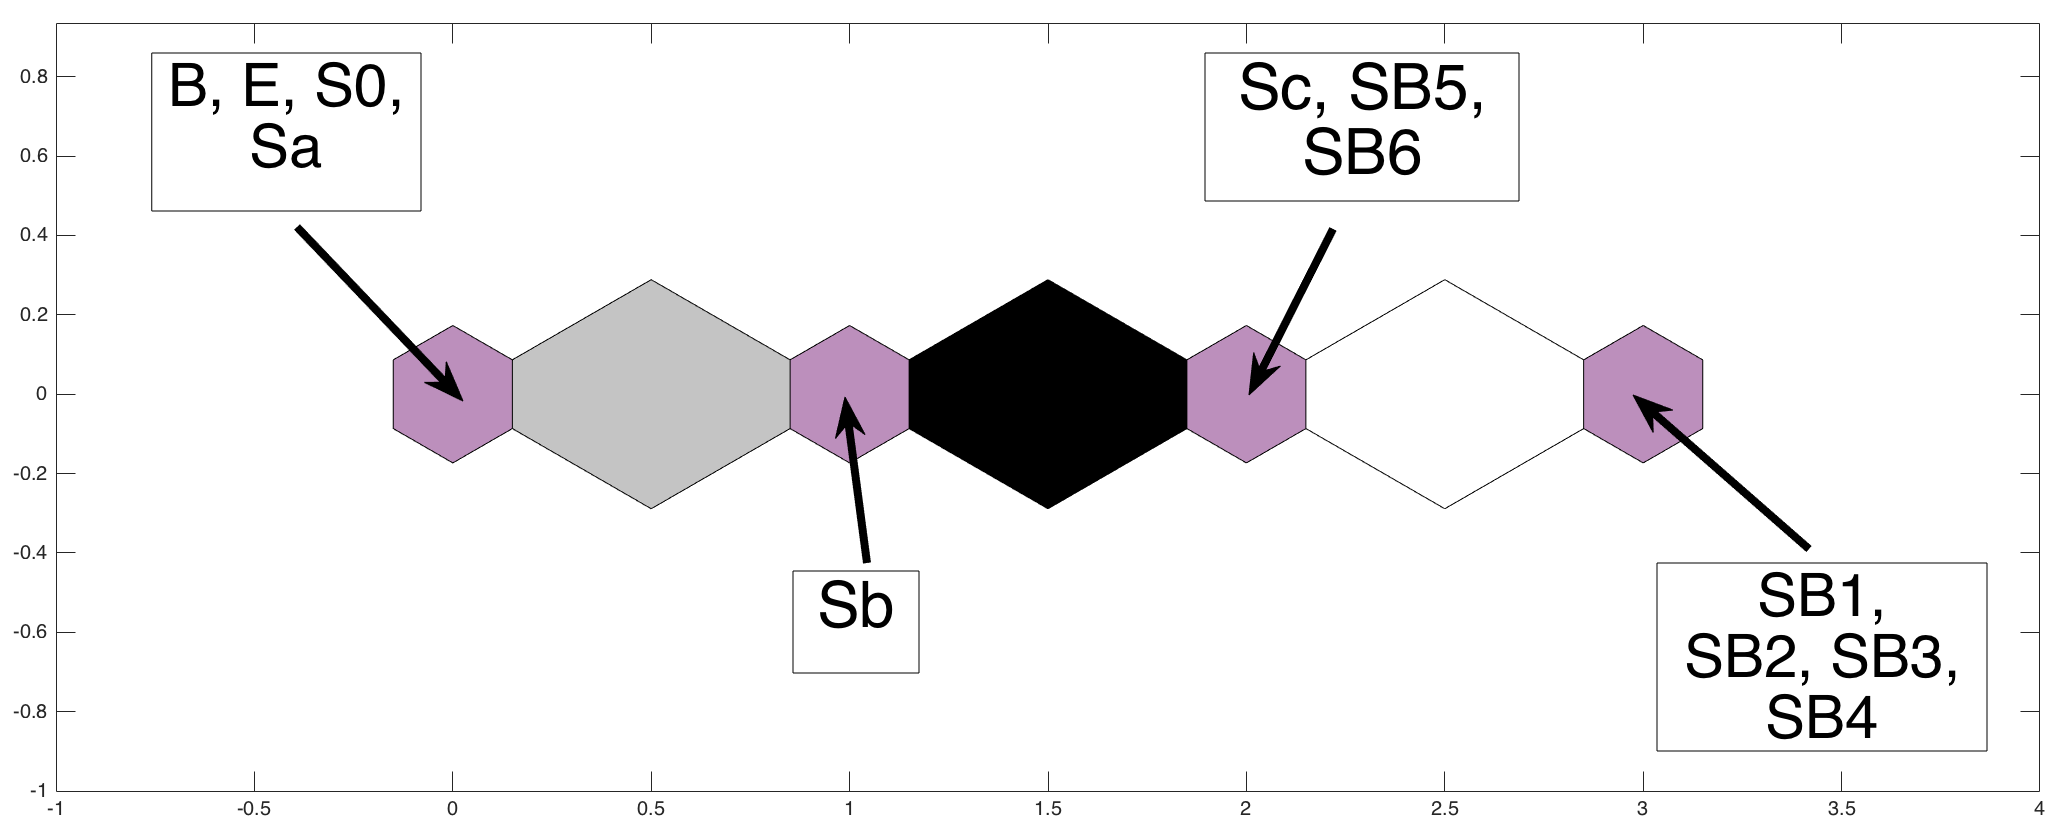
\includegraphics[width=\textwidth]{../images0.01/1d/apps/dist_1_by_4.png}
            %\caption{$1\times4$ weight map}
             %\label{fig: 1by4T}
        \end{subfigure}
        \hfill
        \begin{subfigure}[b]{0.5\textwidth}
             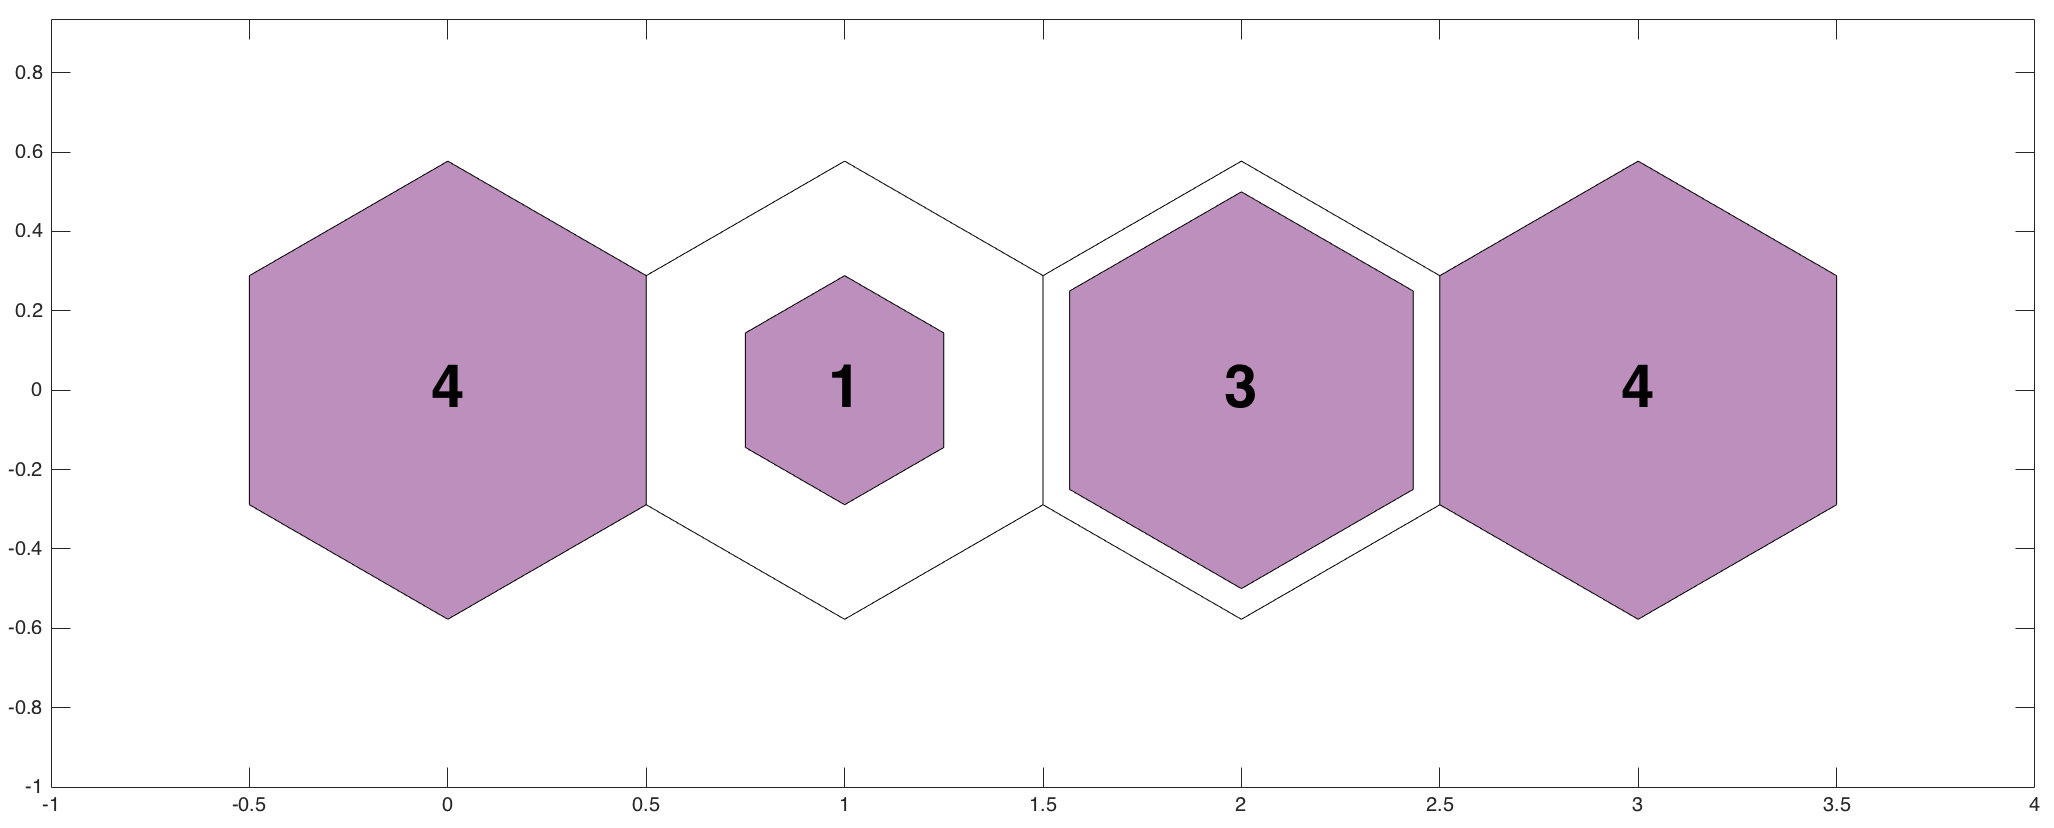
\includegraphics[width=\textwidth]{../images0.01/1d/apps/hit_t_1_by_4.png}
             %\caption{$1\times4$ hits map}
             %\label{fig: 1by4Thits}
        \end{subfigure}
                \caption{Results of training network in $1\times4$~grid.}
         \label{fig: 1by4T}
    \end{figure}
    
    \begin{figure}
        \begin{subfigure}[b]{0.5\textwidth}
            \centering
            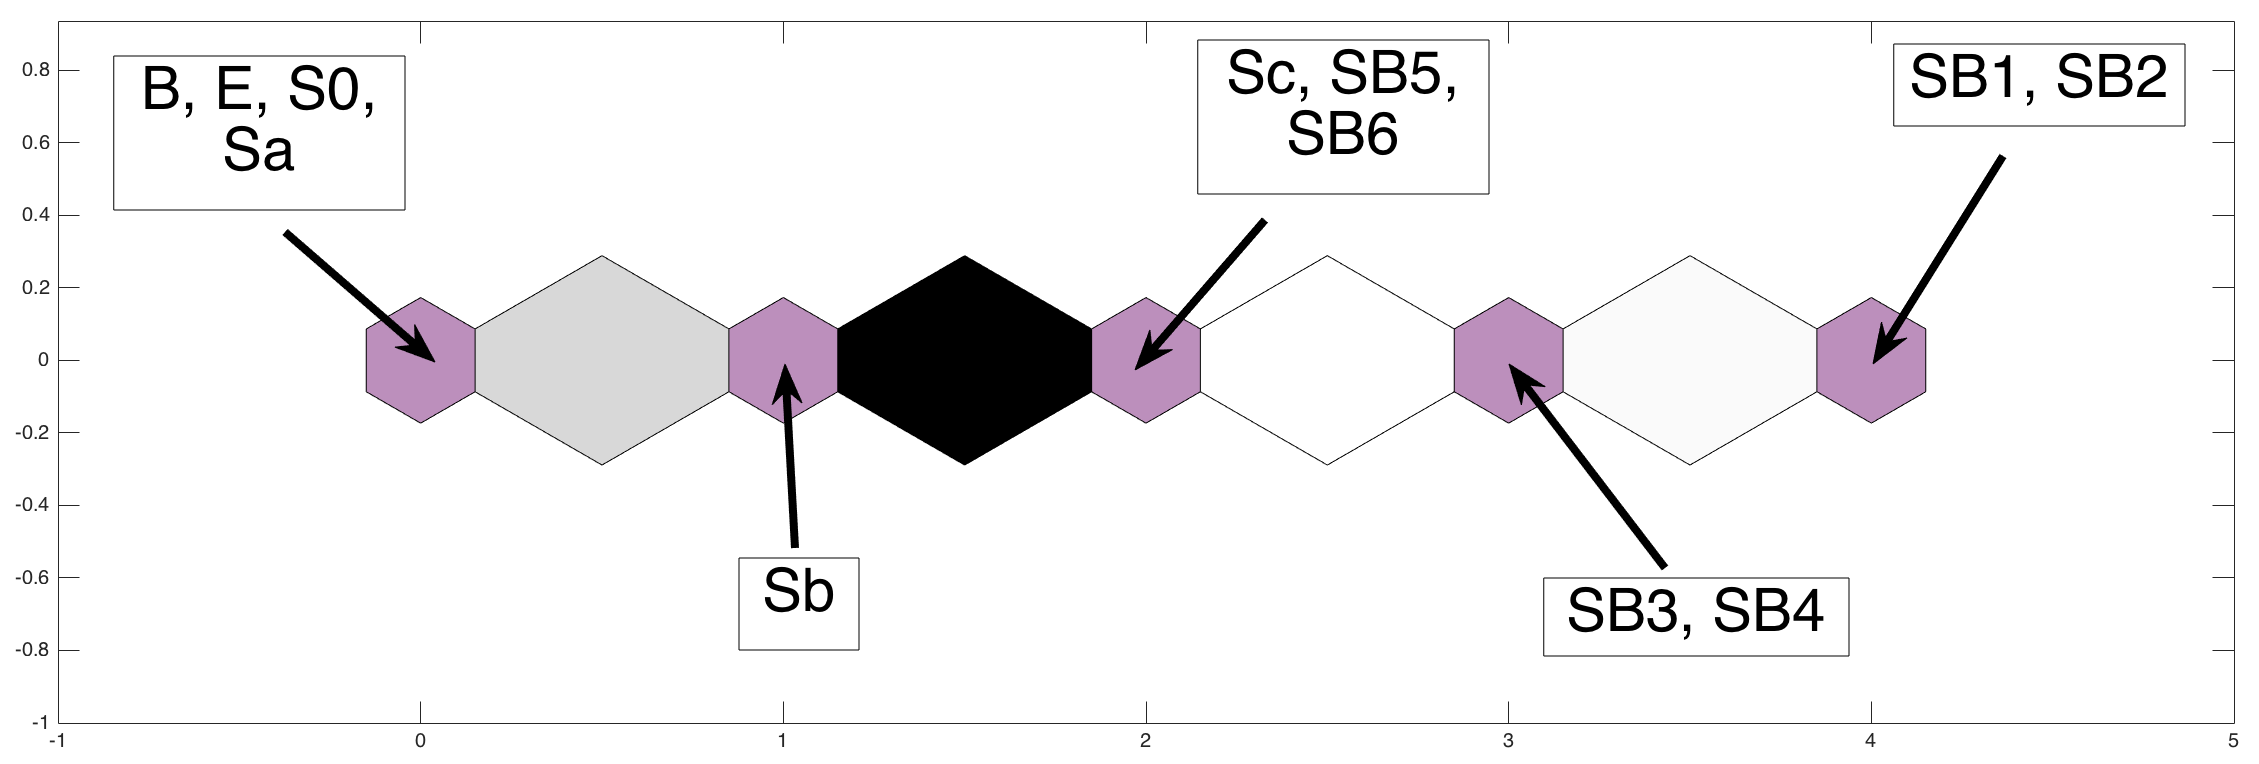
\includegraphics[width=\textwidth]{../images0.01/1d/apps/dist_1_by_5.png}
            %\caption{$1\times5$ weight map}
             %\label{fig: 1by5T}
        \end{subfigure}
        \hfill
        \begin{subfigure}[b]{0.5\textwidth}
             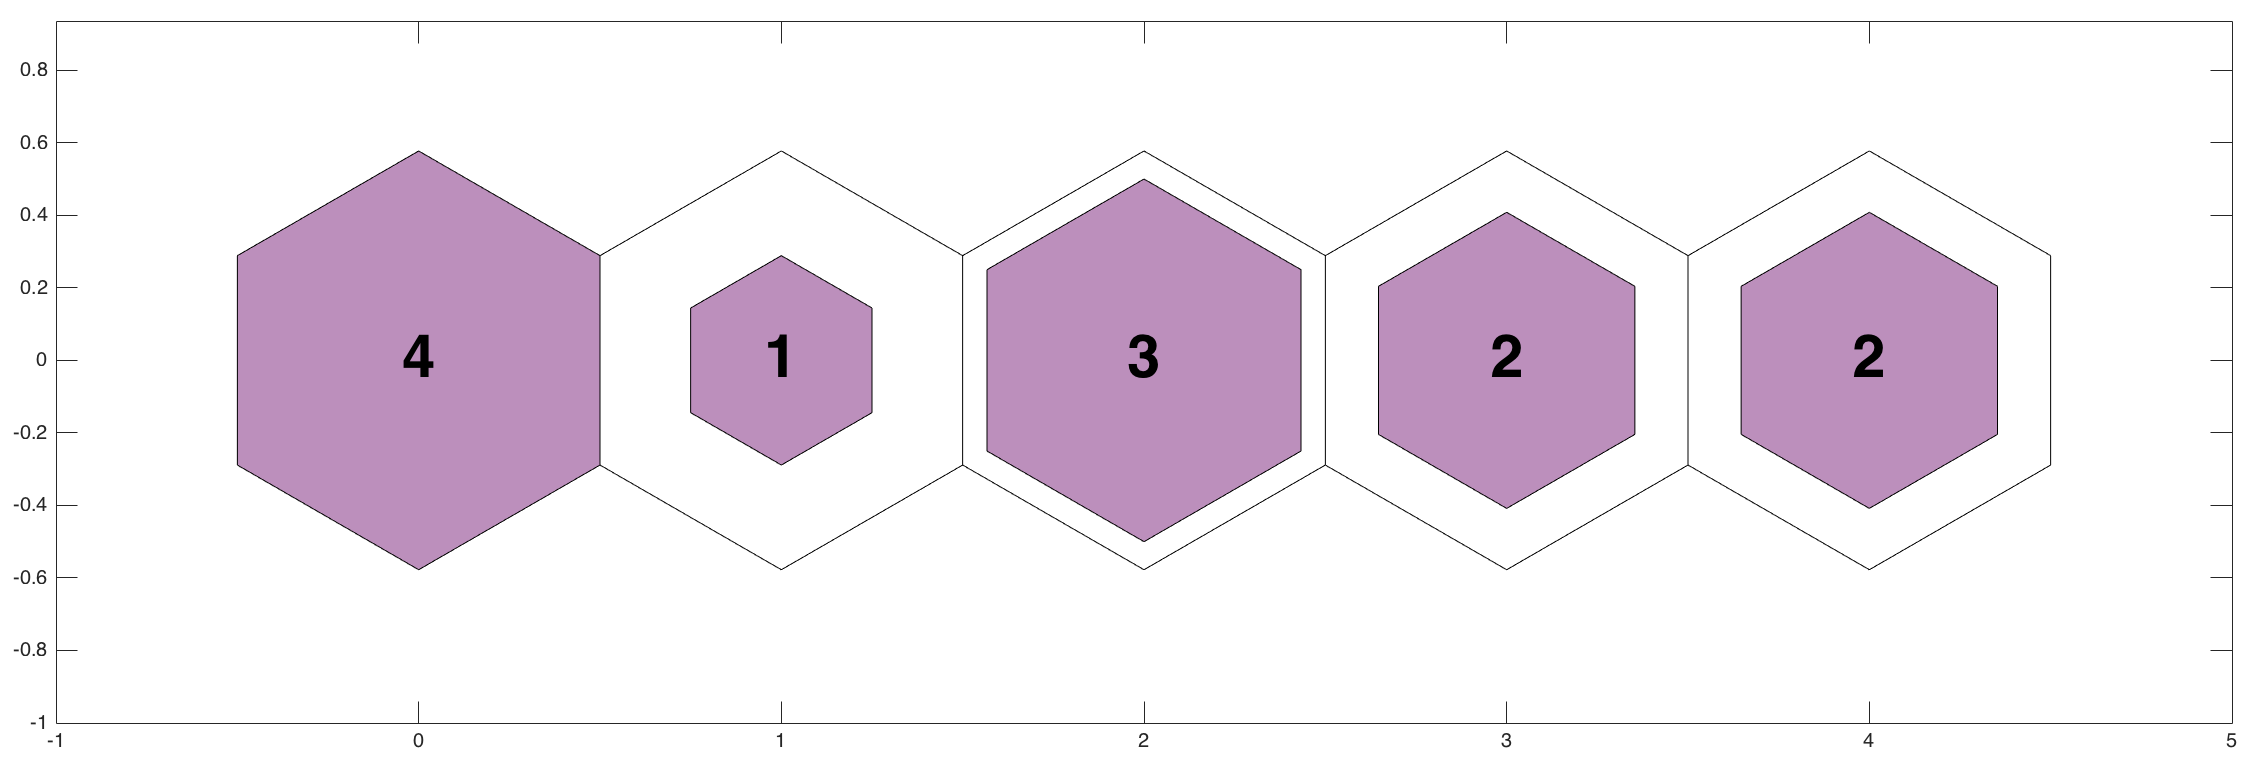
\includegraphics[width=\textwidth]{../images0.01/1d/apps/hit_t_1_by_5.png}
             %\caption{$1\times5$ hits map}
             %\label{fig: 1by5Thits}
        \end{subfigure}
                \caption{Results of training network in $1\times5$~grid.}
         \label{fig: 1by5T}
    \end{figure}
    
    \begin{figure}
        \begin{subfigure}[b]{0.5\textwidth}
            \centering
            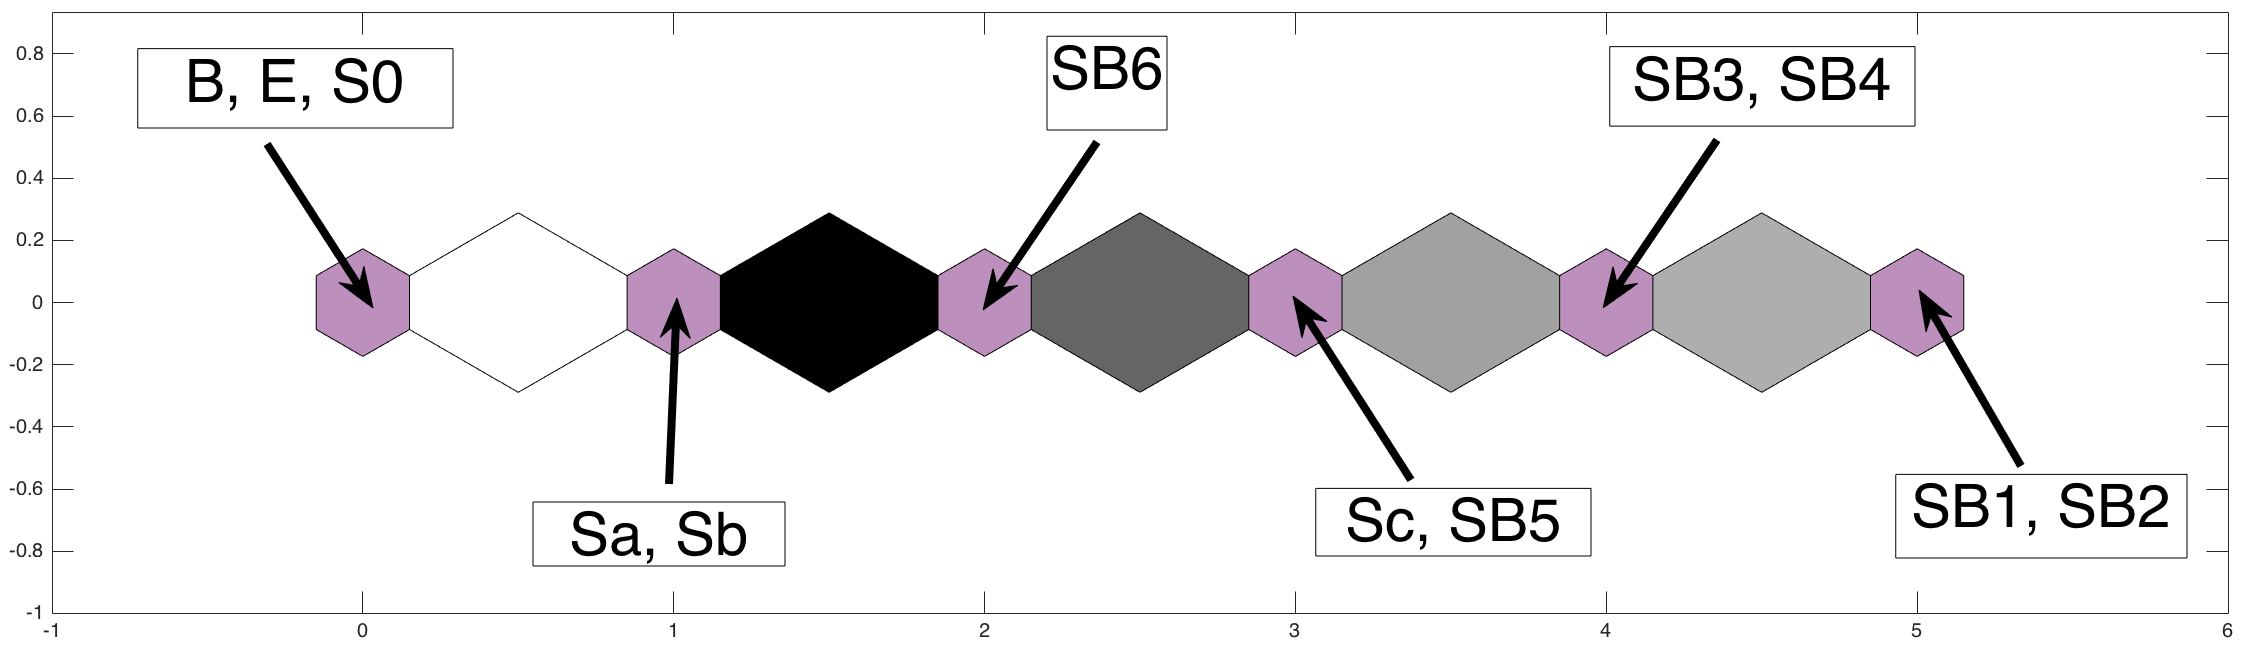
\includegraphics[width=\textwidth]{../images0.01/1d/apps/dist_1_by_6.png}
            %\caption{$1\times6$ weight map}
             %\label{fig: 1by6T}
        \end{subfigure}
        \hfill
        \begin{subfigure}[b]{0.5\textwidth}
             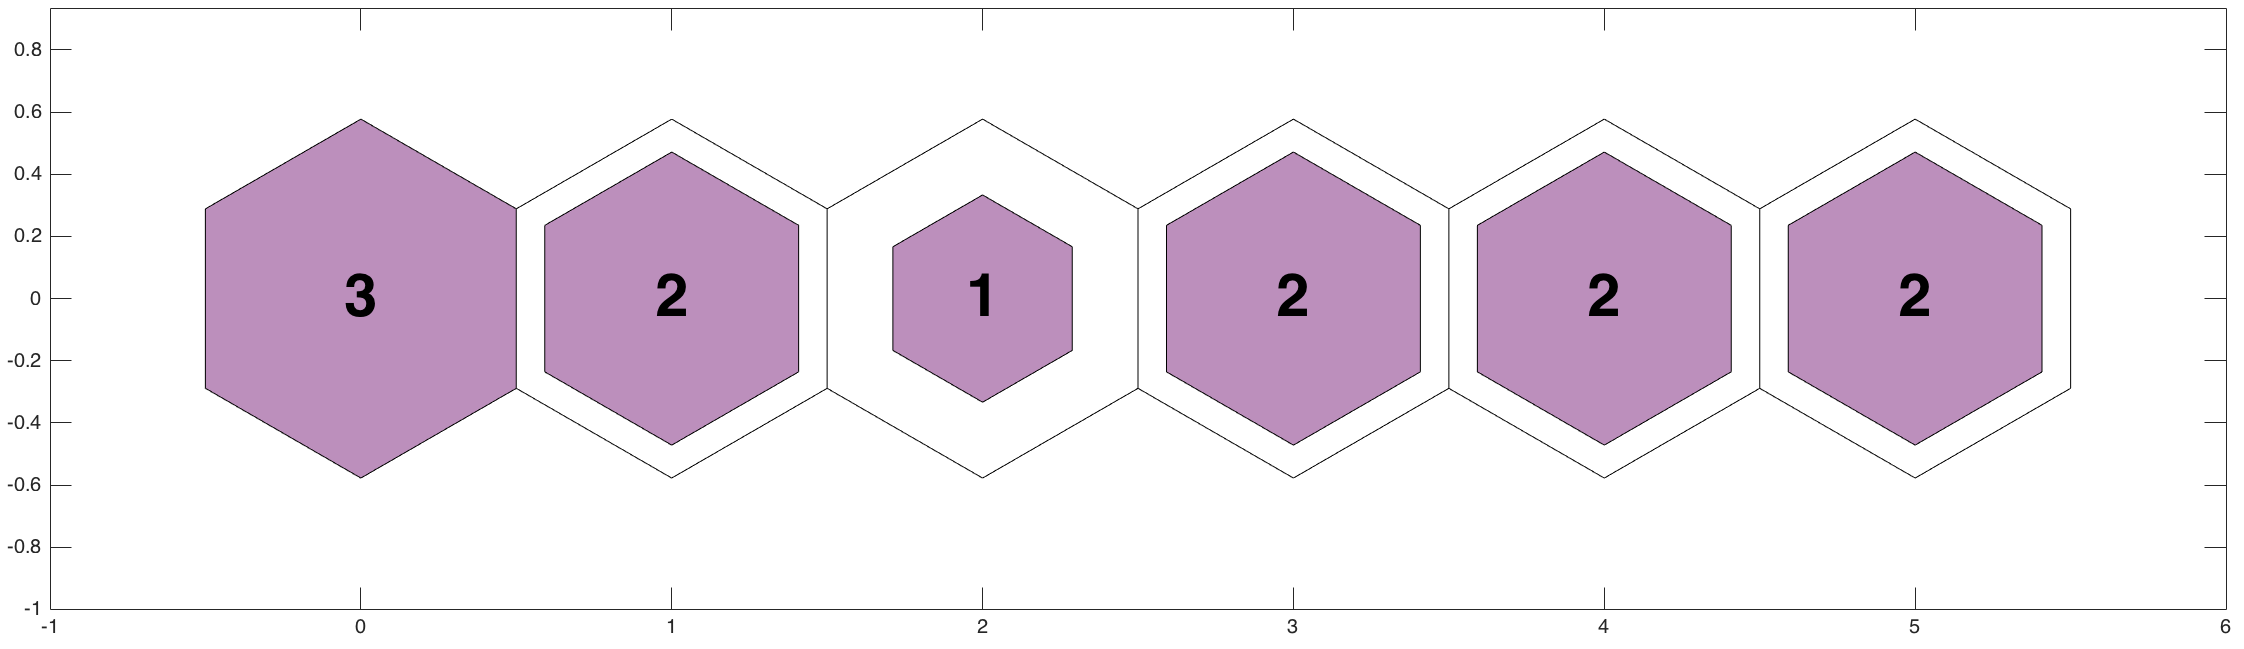
\includegraphics[width=\textwidth]{../images0.01/1d/apps/hit_t_1_by_6.png}
             %\caption{$1\times6$ hits map}
             %\label{fig: 1by6Thits}
        \end{subfigure}
                \caption{Results of training network in $1\times6$~grid.}
         \label{fig: 1by6T}
    \end{figure}
    
    \begin{figure}
        \begin{subfigure}[b]{0.5\textwidth}
            \centering
            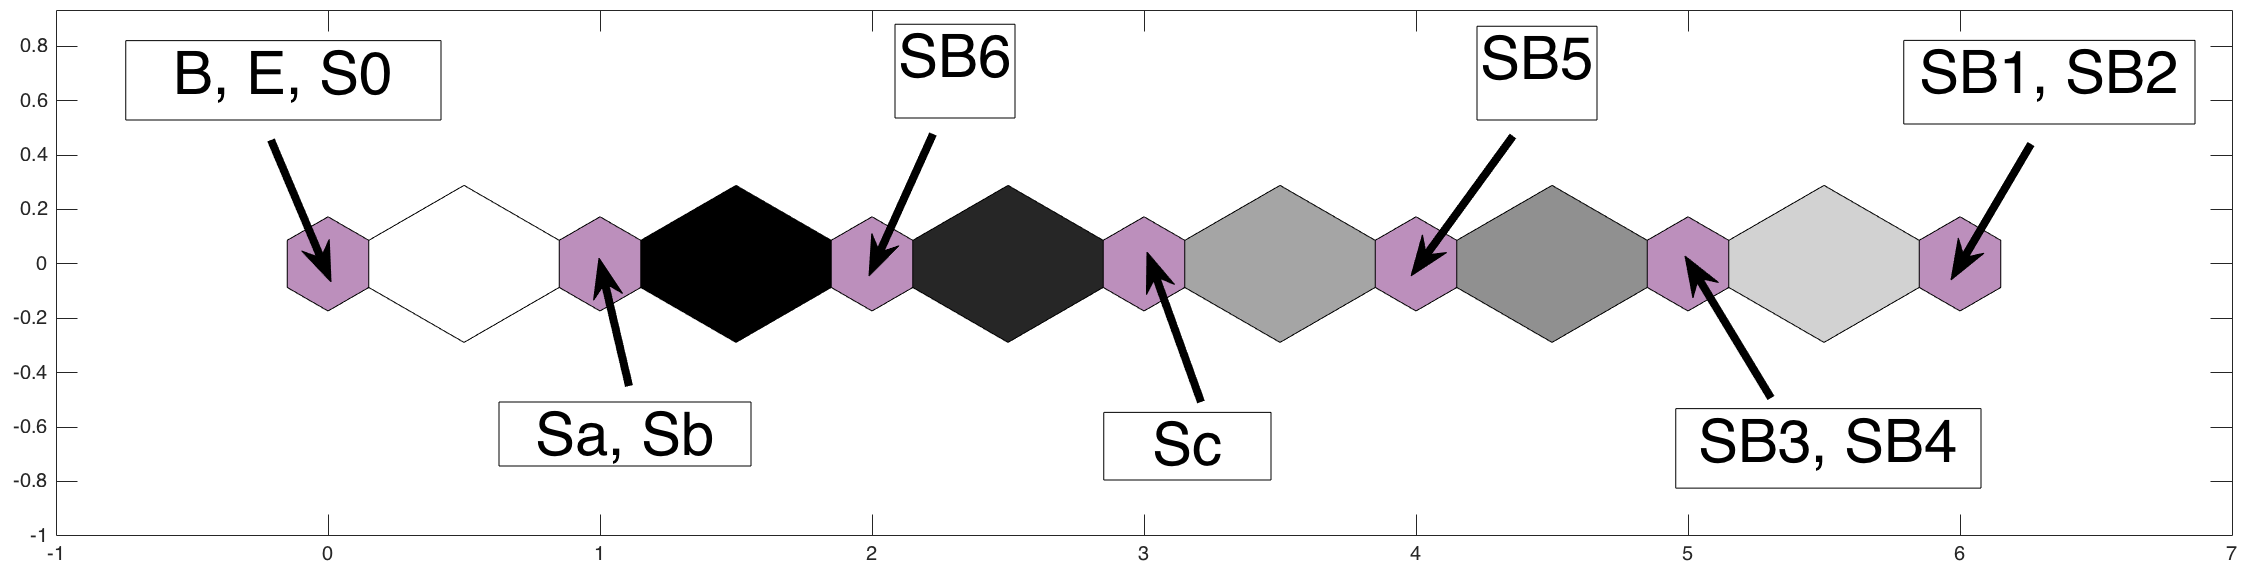
\includegraphics[width=\textwidth]{../images0.01/1d/apps/dist_1_by_7.png}
            %\caption{$1\times7$ weight map}
             %\label{fig: 1by7T}
        \end{subfigure}
        \hfill
        \begin{subfigure}[b]{0.5\textwidth}
             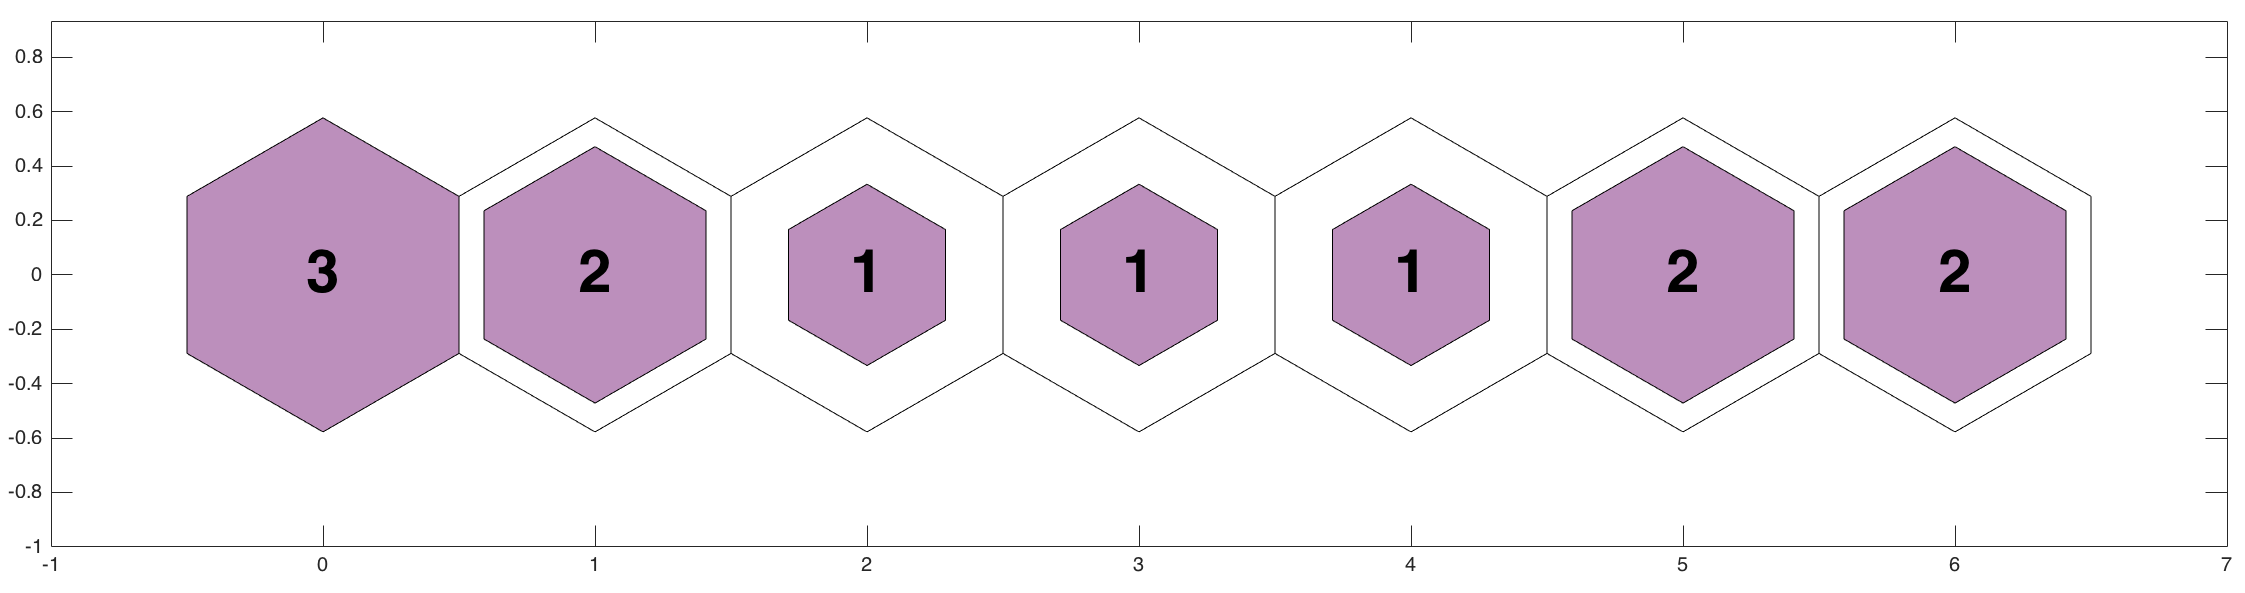
\includegraphics[width=\textwidth]{../images0.01/1d/apps/hit_t_1_by_7.png}
             %\caption{$1\times7$ hits map}
             %\label{fig: 1by7Thits}
        \end{subfigure}
                \caption{Results of training network in $1\times7$~grid.}
         \label{fig: 1by7T}
    \end{figure}
    
    \begin{figure}
        \begin{subfigure}[b]{0.5\textwidth}
            \centering
            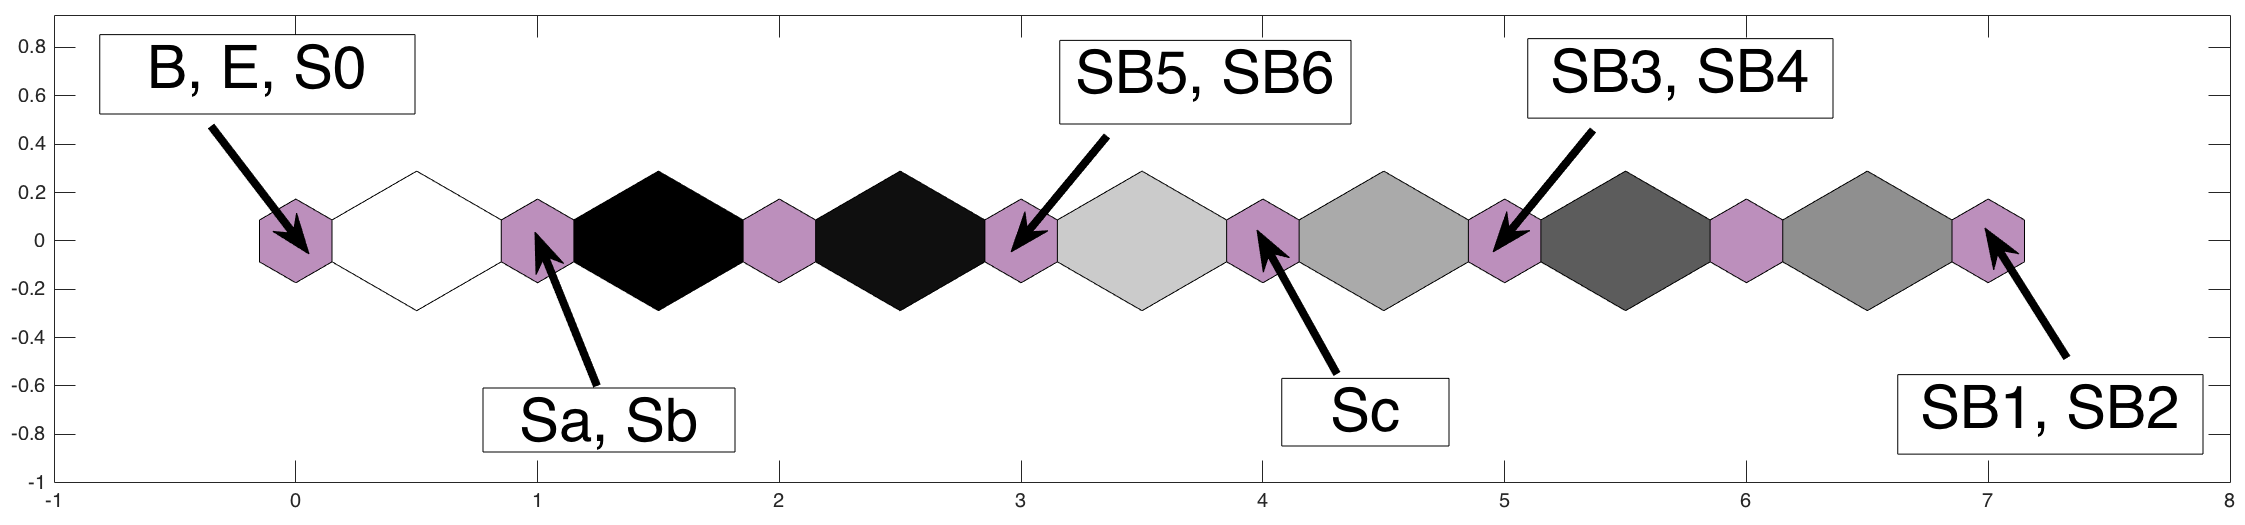
\includegraphics[width=\textwidth]{../images0.01/1d/apps/dist_1_by_8.png}
            %\caption{$1\times8$ weight map}
             %\label{fig: 1by8T}
        \end{subfigure}
        \hfill
        \begin{subfigure}[b]{0.5\textwidth}
             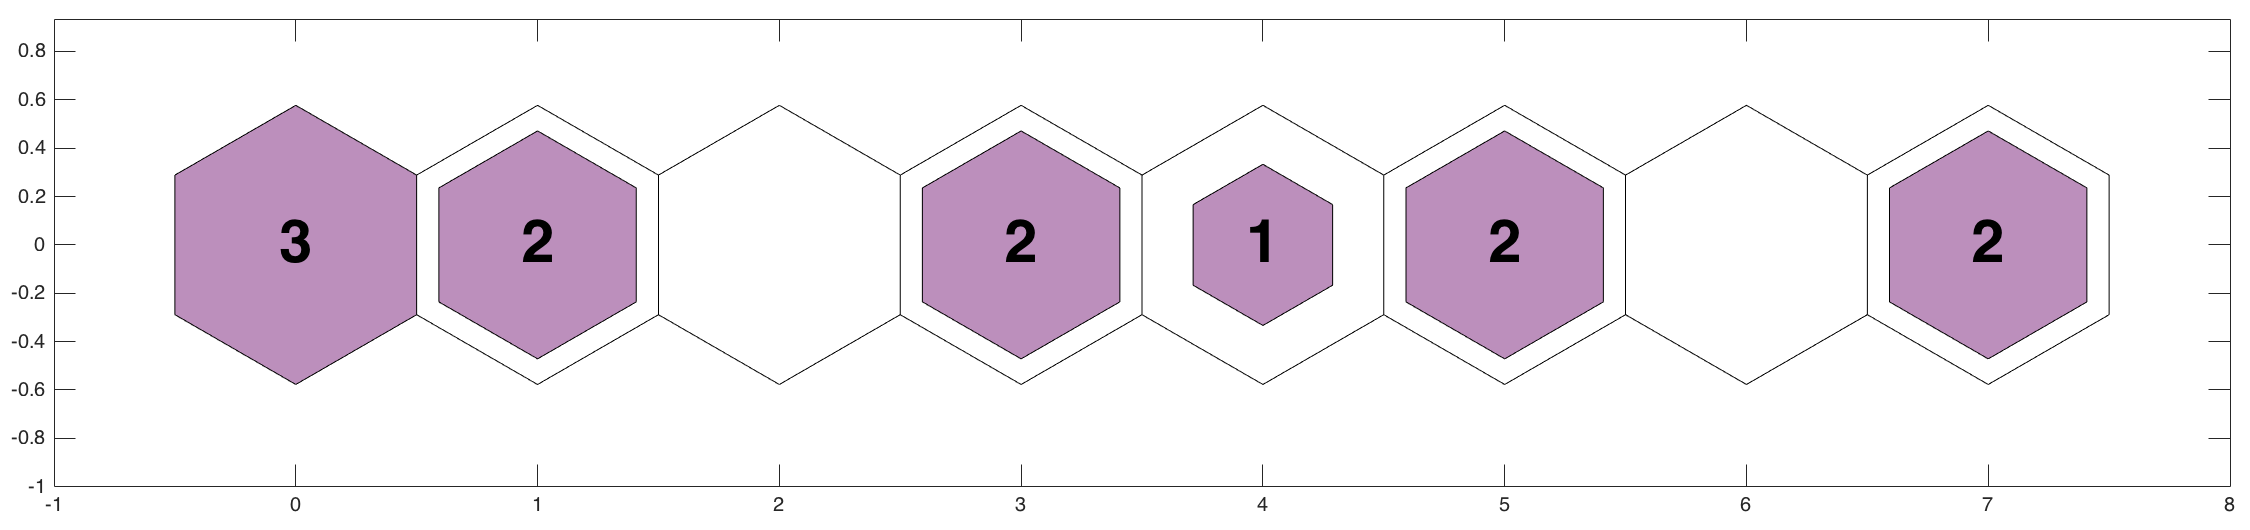
\includegraphics[width=\textwidth]{../images0.01/1d/apps/hit_t_1_by_8.png}
             %\caption{$1\times8$ hits map}
             %\label{fig: 1by8Thits}
        \end{subfigure}
                \caption{Results of training network in $1\times8$~grid.}
         \label{fig: 1by8T}
    \end{figure}
    
    \begin{figure}
        \begin{subfigure}[b]{0.5\textwidth}
            \centering
            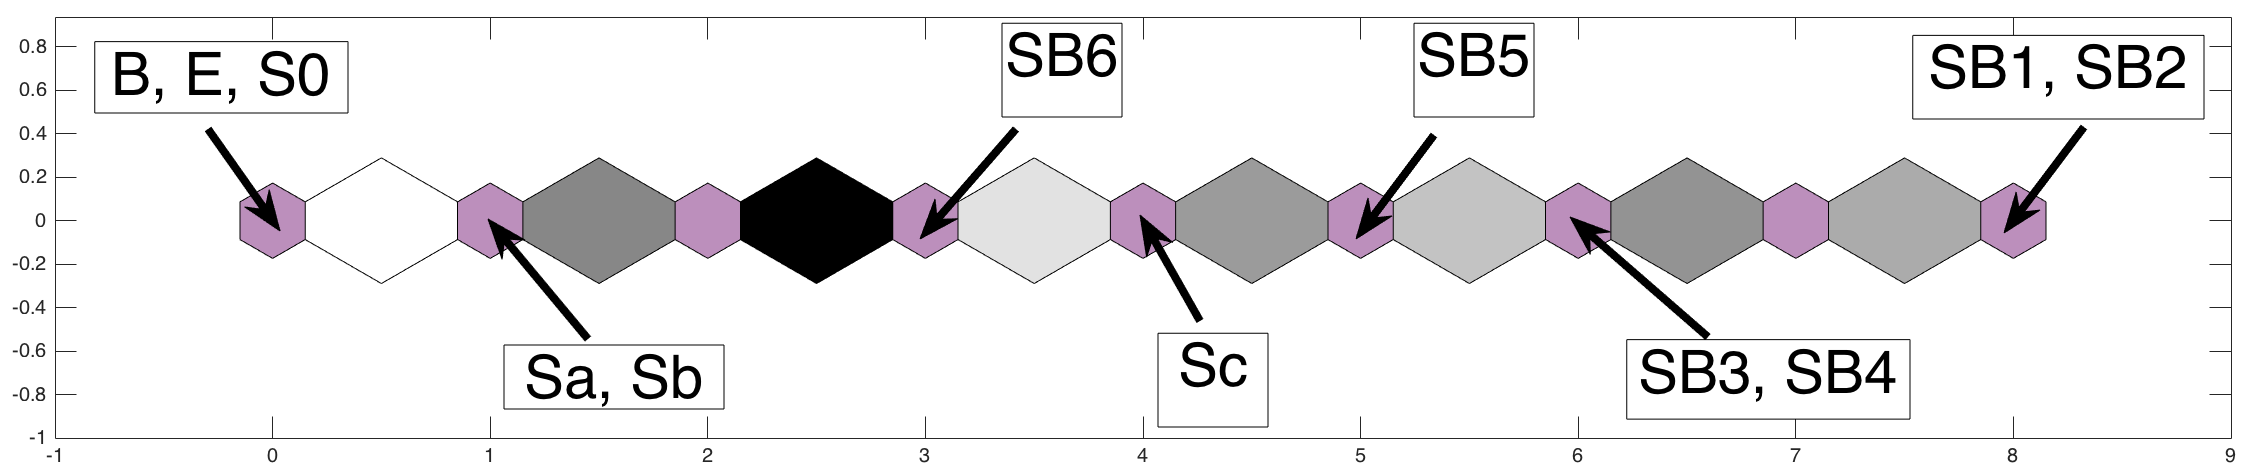
\includegraphics[width=\textwidth]{../images0.01/1d/apps/dist_1_by_9.png}
            %\caption{$1\times9$ weight map}
             %\label{fig: 1by9T}
        \end{subfigure}
        \hfill
        \begin{subfigure}[b]{0.5\textwidth}
             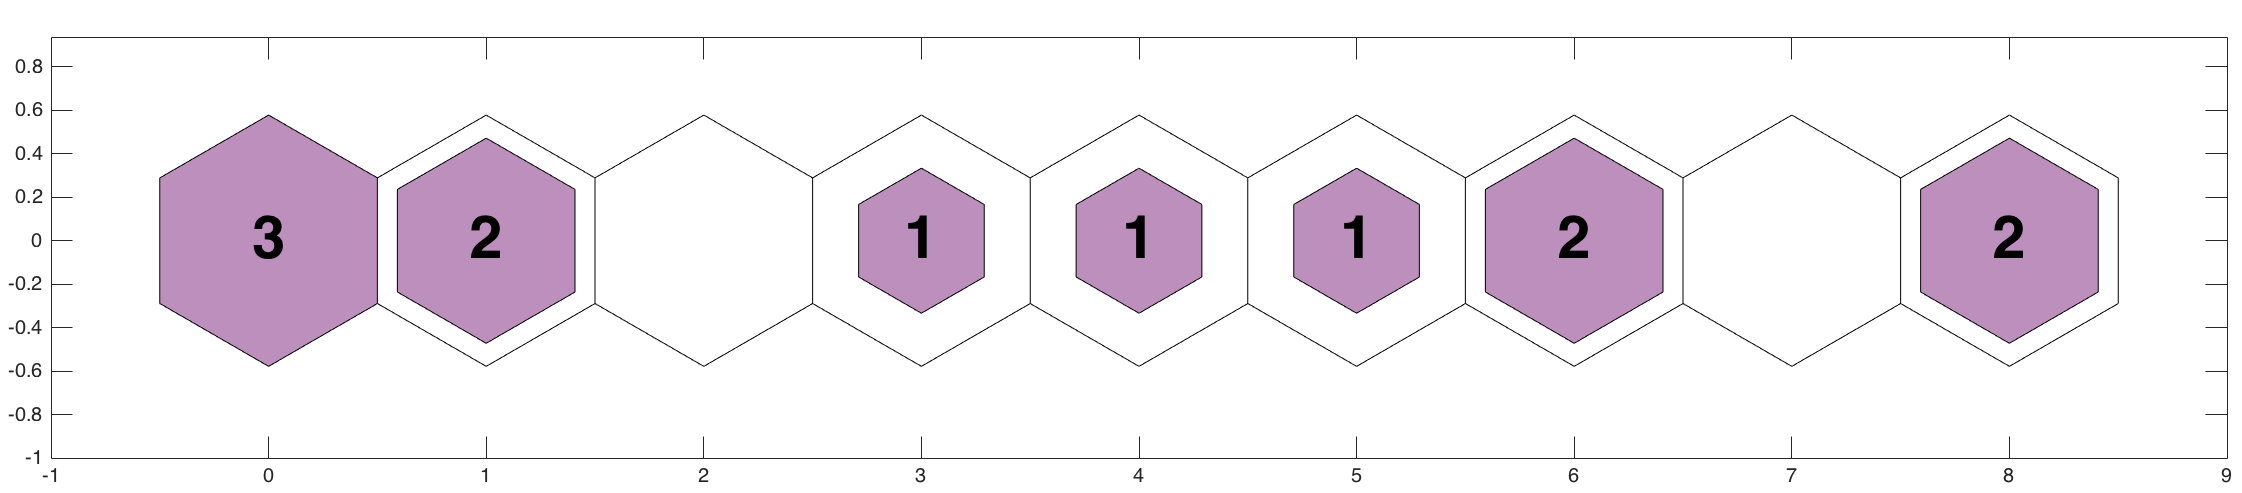
\includegraphics[width=\textwidth]{../images0.01/1d/apps/hit_t_1_by_9.png}
             %\caption{$1\times9$ hits map}
             %\label{fig: 1by9Thits}
        \end{subfigure}
                \caption{Results of training network in $1\times9$~grid.}
         \label{fig: 1by9T}
    \end{figure}

    \begin{figure}
        \begin{subfigure}[b]{0.5\textwidth}
            \centering
            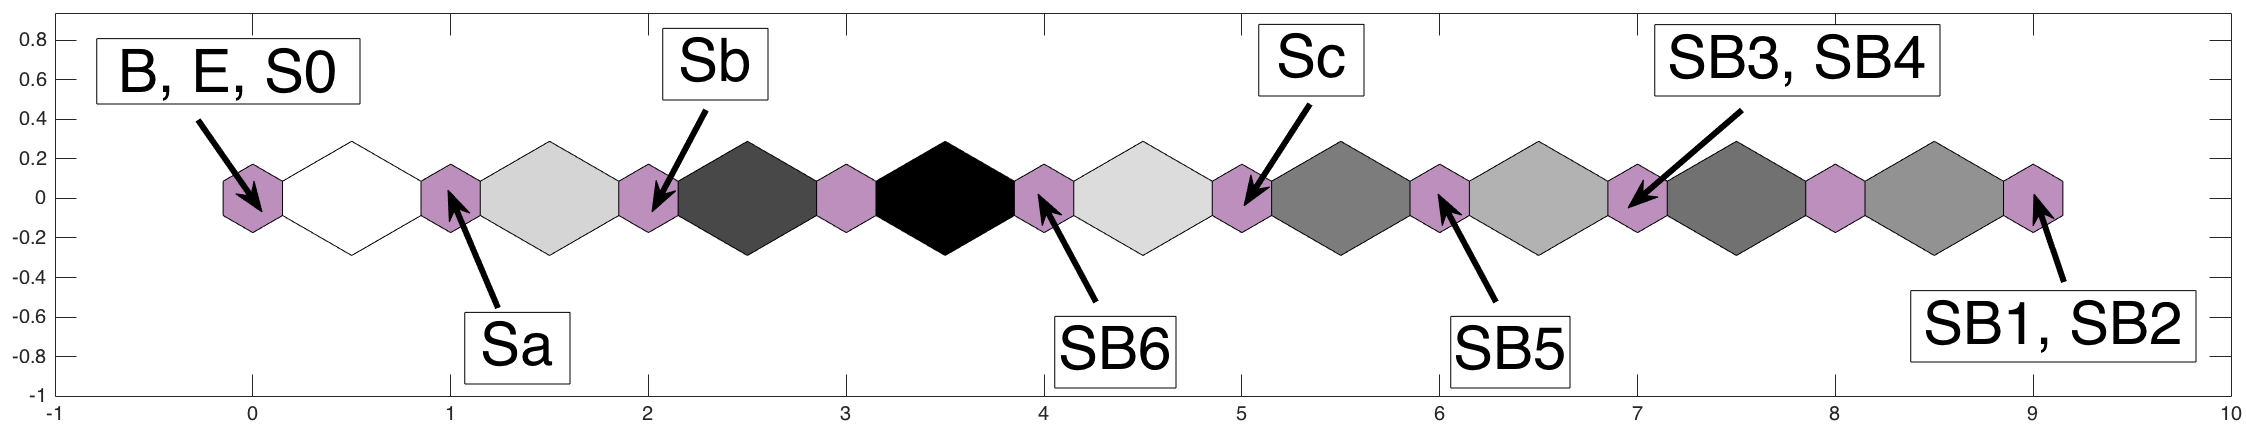
\includegraphics[width=\textwidth,height=2.5cm]{../images0.01/1d/apps/dist_1_by_10.png}
            %\caption{$1\times10$ weight map}
             %\label{fig: 1by10T}
        \end{subfigure}
        \hfill
        \begin{subfigure}[b]{0.5\textwidth}
             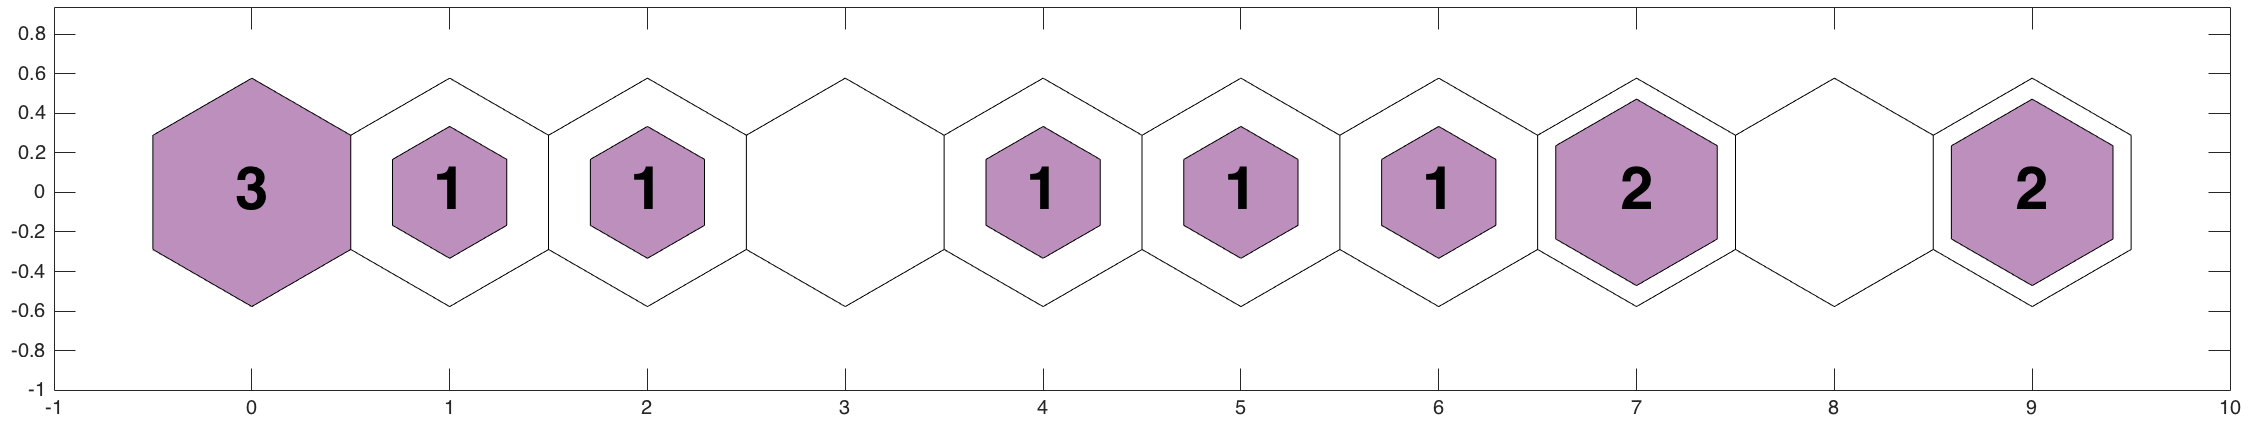
\includegraphics[width=\textwidth,height=2.5cm]{../images0.01/1d/apps/hit_t_1_by_10.png}
             %\caption{$1\times10$ hits map}
             %\label{fig: 1by10Thits}
        \end{subfigure}
                \caption{Results of training network in $1\times10$~grid.}
         \label{fig: 1by10T}
    \end{figure}

    \begin{figure}
        \begin{subfigure}[b]{0.5\textwidth}
            \centering
            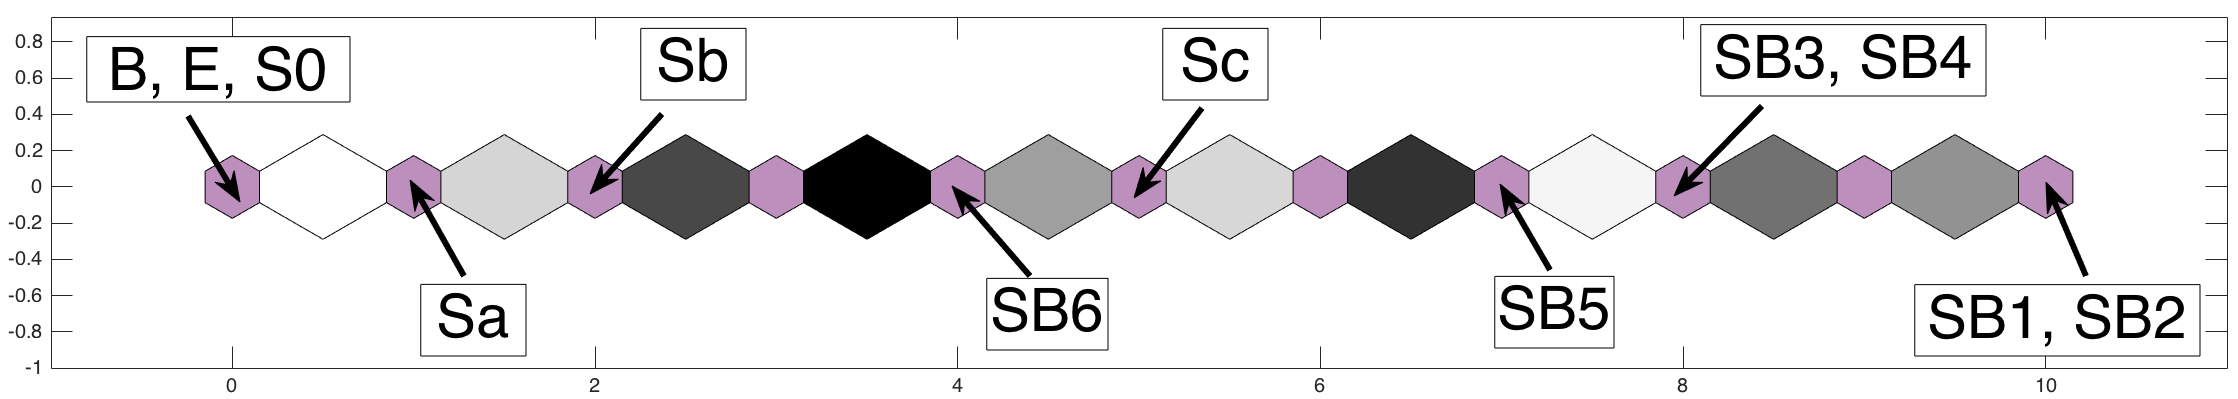
\includegraphics[width=\textwidth,height=2.5cm]{../images0.01/1d/apps/dist_1_by_11.png}
            %\caption{$1\times11$ weight map}
             %\label{fig: 1by11T}
        \end{subfigure}
        \hfill
        \begin{subfigure}[b]{0.5\textwidth}
             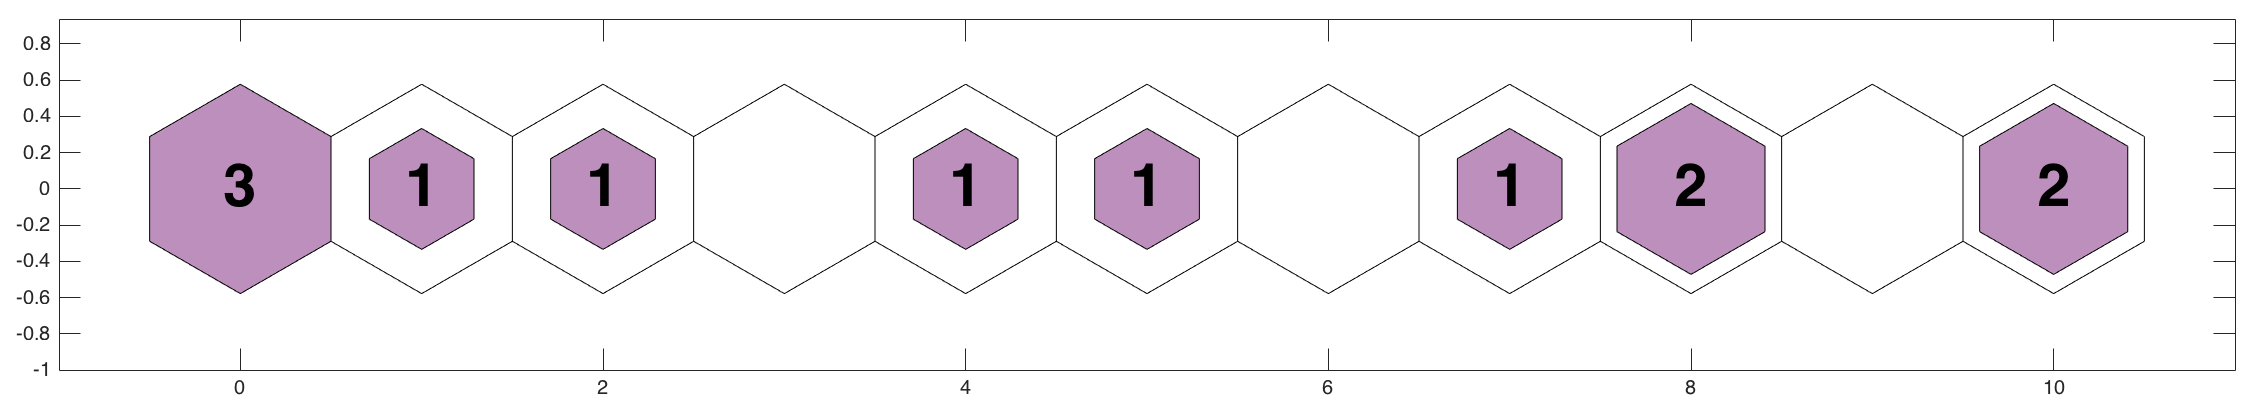
\includegraphics[width=\textwidth,height=2.5cm]{../images0.01/1d/apps/hit_t_1_by_11.png}
             %\caption{$1\times11$ hits map}
             %\label{fig: 1by11Thits}
        \end{subfigure}
                \caption{Results of training network in $1\times11$~grid.}
         \label{fig: 1by11T}
    \end{figure}
    

    \begin{figure}
        \begin{subfigure}[b]{0.5\textwidth}
            \centering
            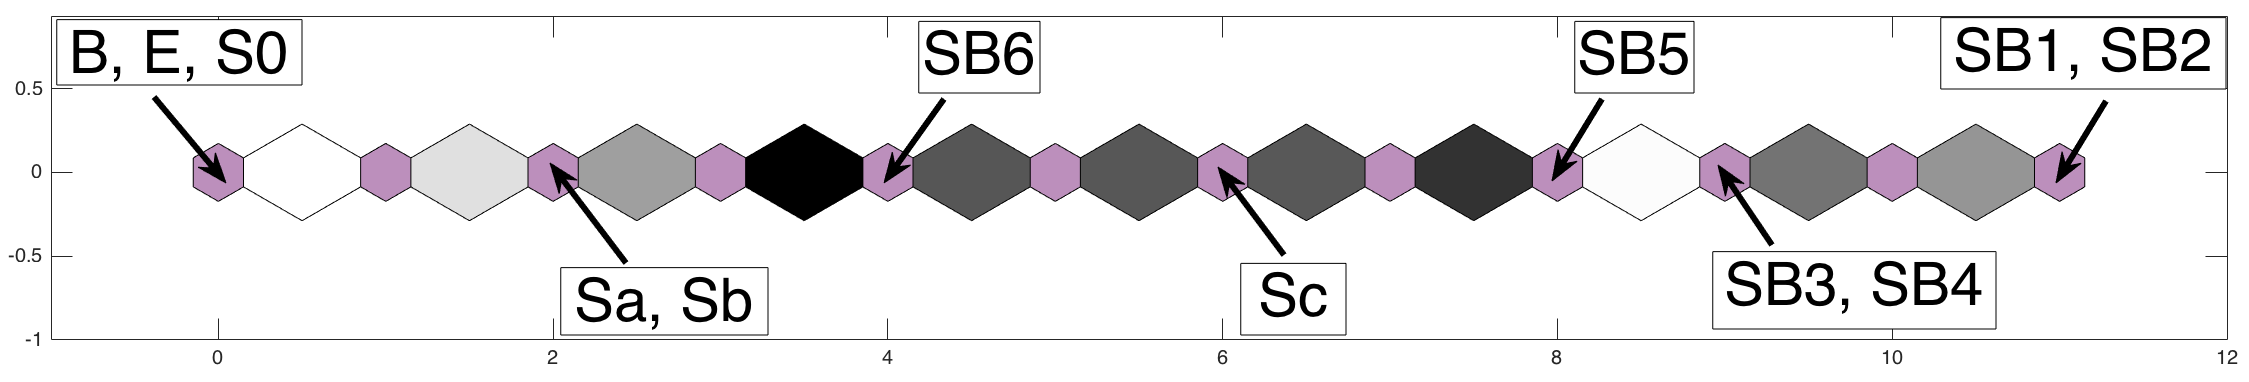
\includegraphics[width=\textwidth,height=2.5cm]{../images0.01/1d/apps/dist_1_by_12.png}
            %\caption{$1\times12$ weight map}
             %\label{fig: 1by12T}
        \end{subfigure}
        \hfill
        \begin{subfigure}[b]{0.5\textwidth}
             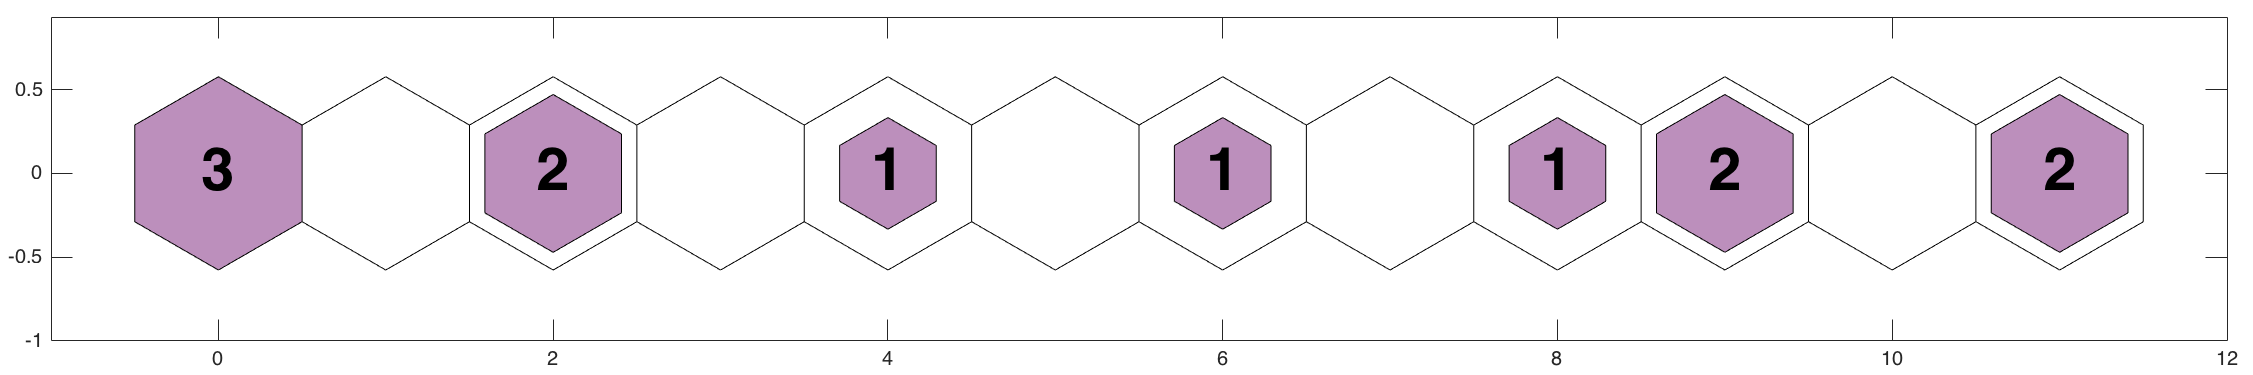
\includegraphics[width=\textwidth,height=2.5cm]{../images0.01/1d/apps/hit_t_1_by_12.png}
             %\caption{$1\times12$ hits map}
             %\label{fig: 1by12Thits}
        \end{subfigure}
                \caption{Results of training network in $1\times12$~grid.}
         \label{fig: 1by12T}
    \end{figure}

    \begin{figure}
        \begin{subfigure}[b]{0.5\textwidth}
            \centering
            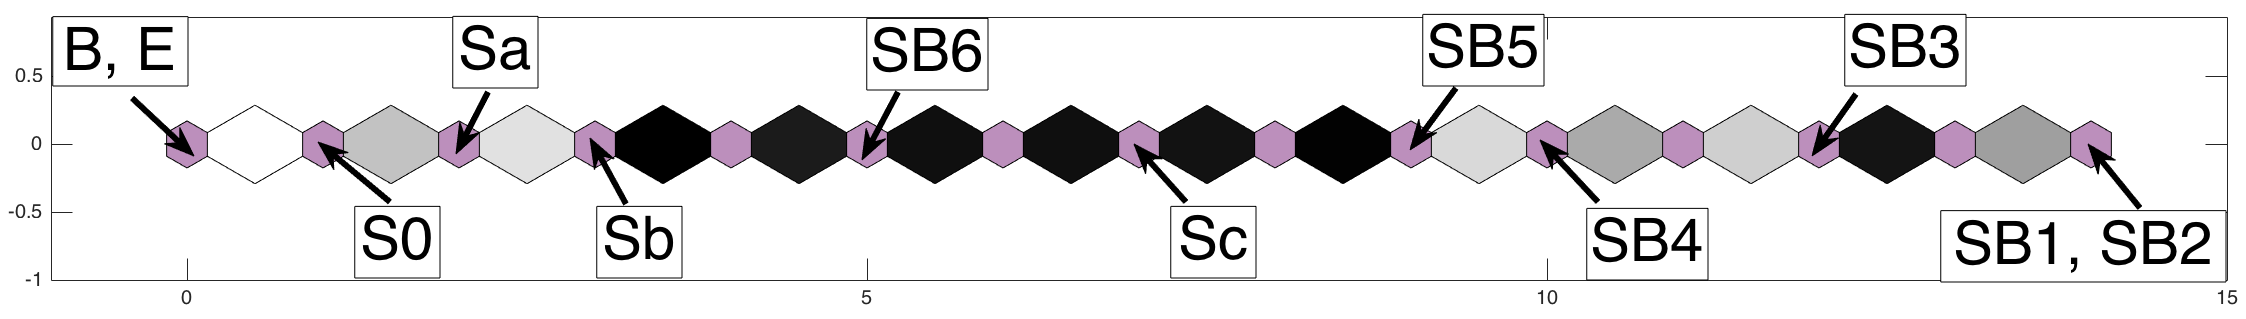
\includegraphics[width=\textwidth,height=2.5cm]{../images0.01/1d/apps/dist_1_by_15.png}
            %\caption{$1\times15$ weight map}
             %\label{fig: 1by15T}
        \end{subfigure}
        \hfill
        \begin{subfigure}[b]{0.5\textwidth}
             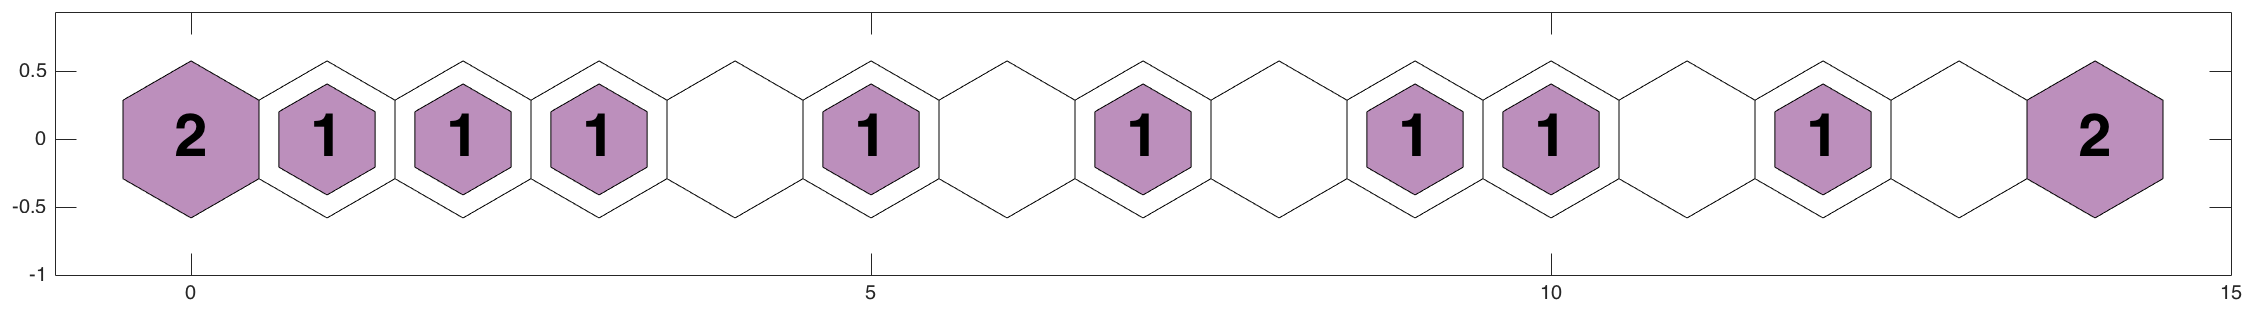
\includegraphics[width=\textwidth,height=2.5cm]{../images0.01/1d/apps/hit_t_1_by_15.png}
             %\caption{$1\times15$ hits map}
             %\label{fig: 1by15Thits}
        \end{subfigure}
                \caption{Results of training network in $1\times15$~grid.}
         \label{fig: 1by15T}
    \end{figure}

    \begin{figure}
        \begin{subfigure}[b]{0.5\textwidth}
            \centering
            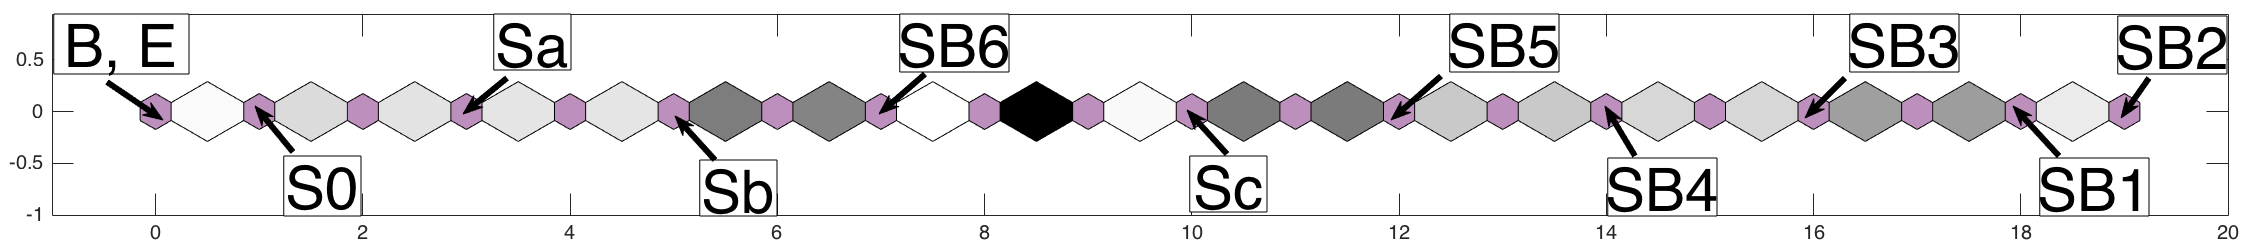
\includegraphics[width=\textwidth,height=2.5cm]{../images0.01/1d/apps/dist_1_by_20.png}
            %\caption{$1\times20$ weight map}
             %\label{fig: 1by20T}
        \end{subfigure}
        \hfill
        \begin{subfigure}[b]{0.5\textwidth}
             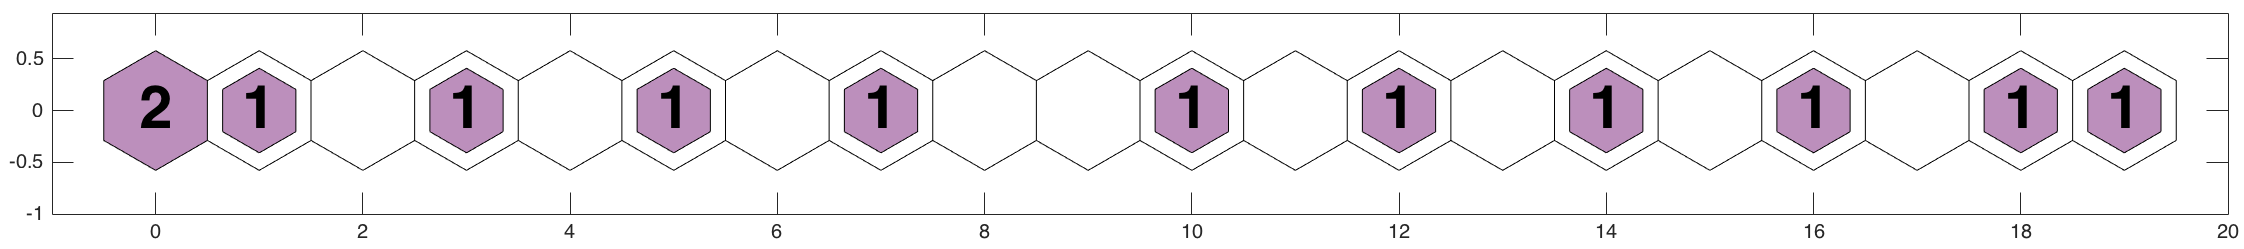
\includegraphics[width=\textwidth,height=2.5cm]{../images0.01/1d/apps/hit_t_1_by_20.png}
             %\caption{$1\times20$ hits map}
             %\label{fig: 1by20Thits}
        \end{subfigure}
                \caption{Results of training network in $1\times20$~grid.}
         \label{fig: 1by20T}
    \end{figure}
    

\newpage



\section{Comparison of the self-organizing maps and K-means methods}
\label{app: high_Z_1d_k-means}


In this section we present the result of applying  K-means clustering method on the the spectra of 142 galaxies from \citetalias{Hossein12}.
K-means clustering, alongside of SOMs are two of main unsupervised methods that are being used in astronomical studies \citep[e.g.][]{DAbrusco12, Aycha16}.
In the K-means methods, the user decides number of cluster, K. 
The algorithm, randomly chooses K random points to be set as a centroid of the clusters.
Then, it finds the data points that are closer to the each assumed centroid and cluster them together.
Mean values of the data points that are assigned to each cluster were calculated and become the new centroid of the cluster. 
The algorithm finds new clusters based on the new centroids and repeats the procedure until it converges. 
We used \textsc{matlab} K-means library to perform the K-means clustering.


The number of clusters in the K-means method is arbitrary and is set by the user.
We performed K-means clustering on the \citetalias{Kinney96} template spectra using 4 clusters and on the \citetalias{Hossein12} 142 sample galaxies using and 22 clusters. 
In this case we can easily compare the results of K-means clustering with 1D SOMs. 
To compare the results, we measured the median of spectra for each cluster both in SOM and K-means results.
To classify the 142 sample galaxies, we calculate the median of the spectra in each cluster, and compare them with the \citetalias{Kinney96} template spectra.
We measured the spectral angle distance between the medians and the template spectra, to find the best match between them as follow:
\begin{equation}
    cos(\theta) = \frac{\sum_{i=1}^{n} s_it_i}{(\sum_{i=1}^{n} s^2_i)^{0.5} (\sum_{i=1}^{n} t^2_i)^{0.5}}
\end{equation}
where $s_i$ and $t_i$ are the ith wavelength of sample and template spectra, respectively. 
$\theta$ is the angle between the spectrum, that the zero value means completely similar and the 180  degree means the completely different spectra. Since $cos(\theta)$, changes between -1 and 1, 1-$cos(\theta)$ would be the easier way to measure and report the (dis-)similarity between two spectra.
The spectrum from the the \citetalias{Kinney96} template that has the most similarity with a median of the cluster, would be assigned to the all galaxies in the cluster
 

\begin{figure*}
                \begin{subfigure}[b]{0.49\textwidth}
                    \centering
                  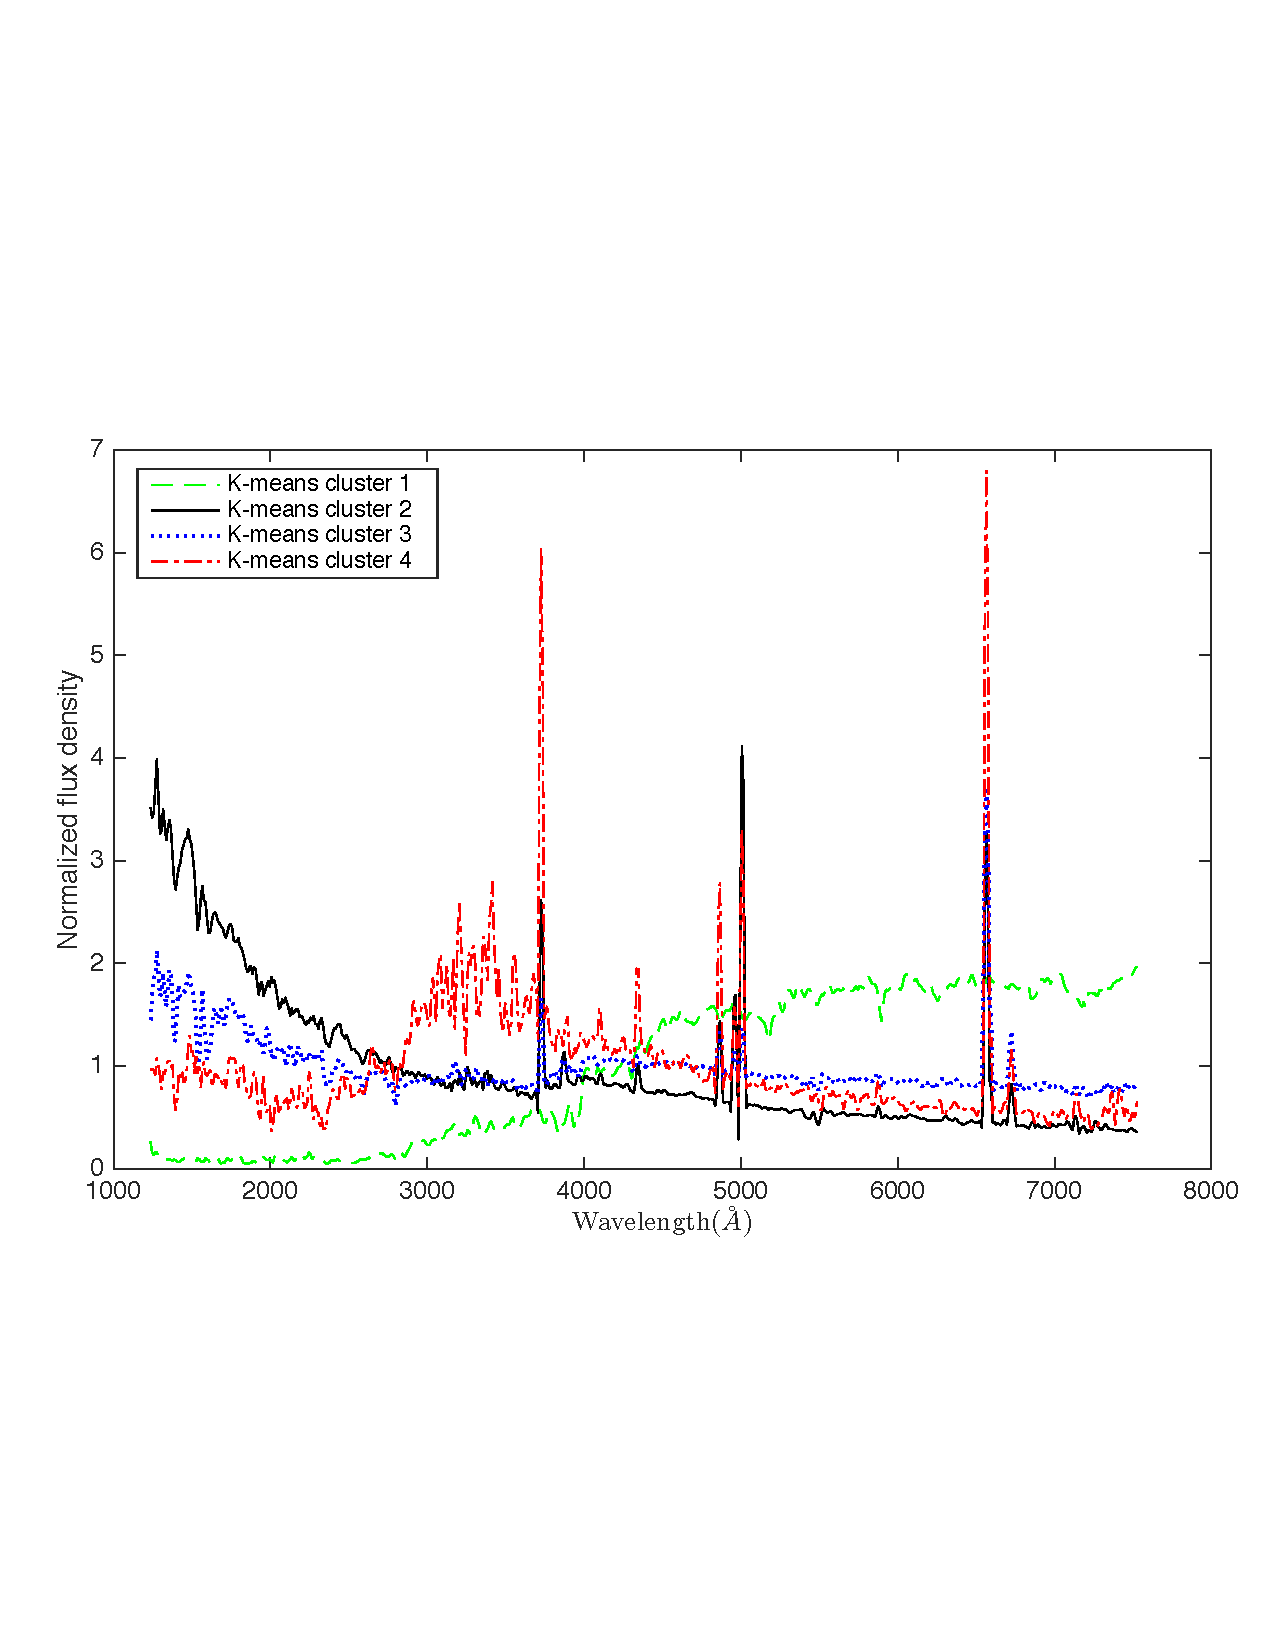
\includegraphics[width=.99\textwidth, height= 7.5cm]{k_means_images/classified_group_in_4cluster.pdf}
                \end{subfigure}
                \hfill
                \begin{subfigure}[b]{0.49\textwidth}
                    \centering 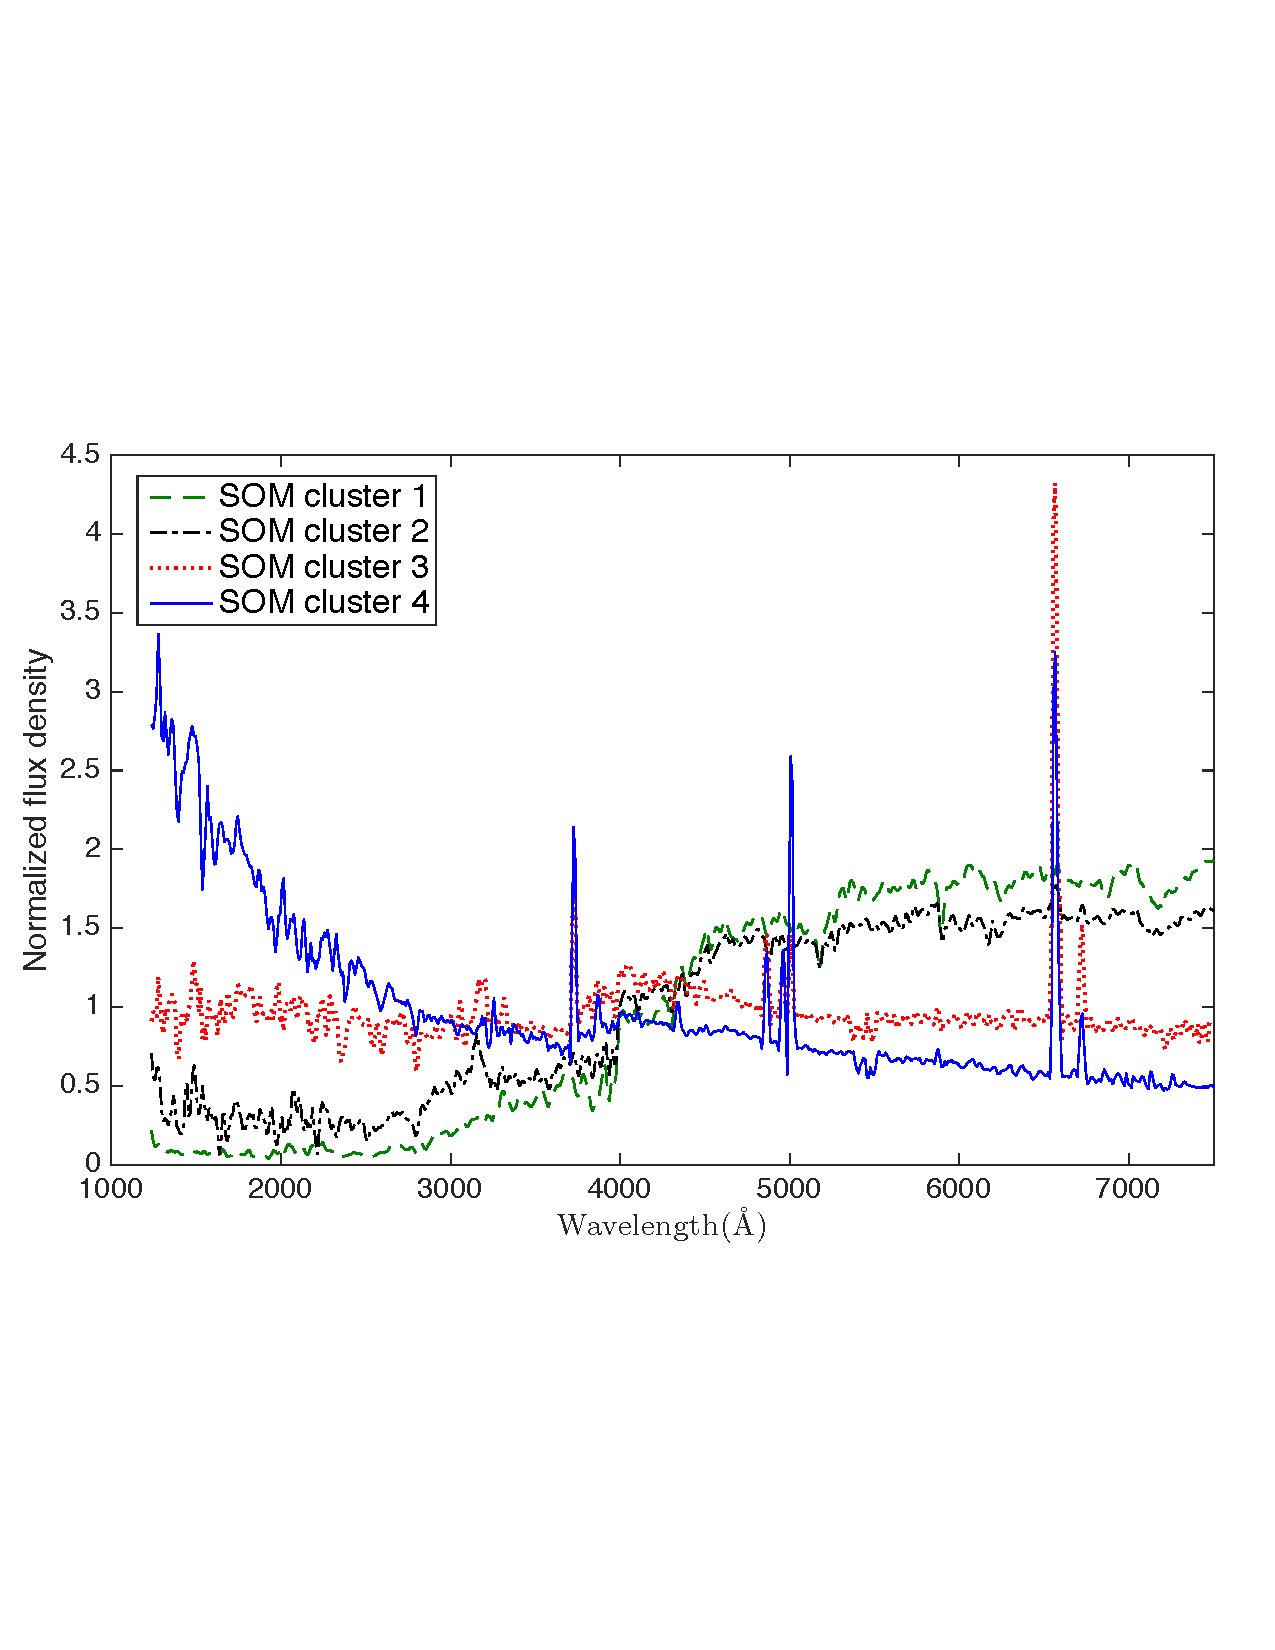
\includegraphics[width=.99\textwidth, height= 7.5cm]{k_means_images/classified_group_in_4cluster_som.pdf}
                \end{subfigure}
                \caption{Clustering the \citetalias{Kinney96} template spectra using K-means clustering (left) and SOM (right). Note that both methods randomly assign the initial values for their analysis, therefore cluster's number is not meaningful and is just for distinction of the clusters.}
                 \label{fig: som_k_means_4}
\end{figure*}
Fig.~\ref{fig: som_k_means_4} shows the clustering of the template spectra in 4 groups using both K-means and SOMs.
For K-means method we cannot have any empty cluster, hence we cannot increase the number of clusters more than 12, which is basically the same as Fig.~\ref{fig: k96}.
Both plots in Fig.~\ref{fig: som_k_means_4}, separated the most starburst and quiescent galaxies in the similar manner.
However, for spectra types between the extreme cases, they show discrepancy. 
The other difference, between these two method is that the network created by SOM method can be used to classify the other spectra, while for the K-means clusters they can only be used one set of data.



\begin{figure*}
                \begin{subfigure}[b]{0.49\textwidth}
                    \centering
                  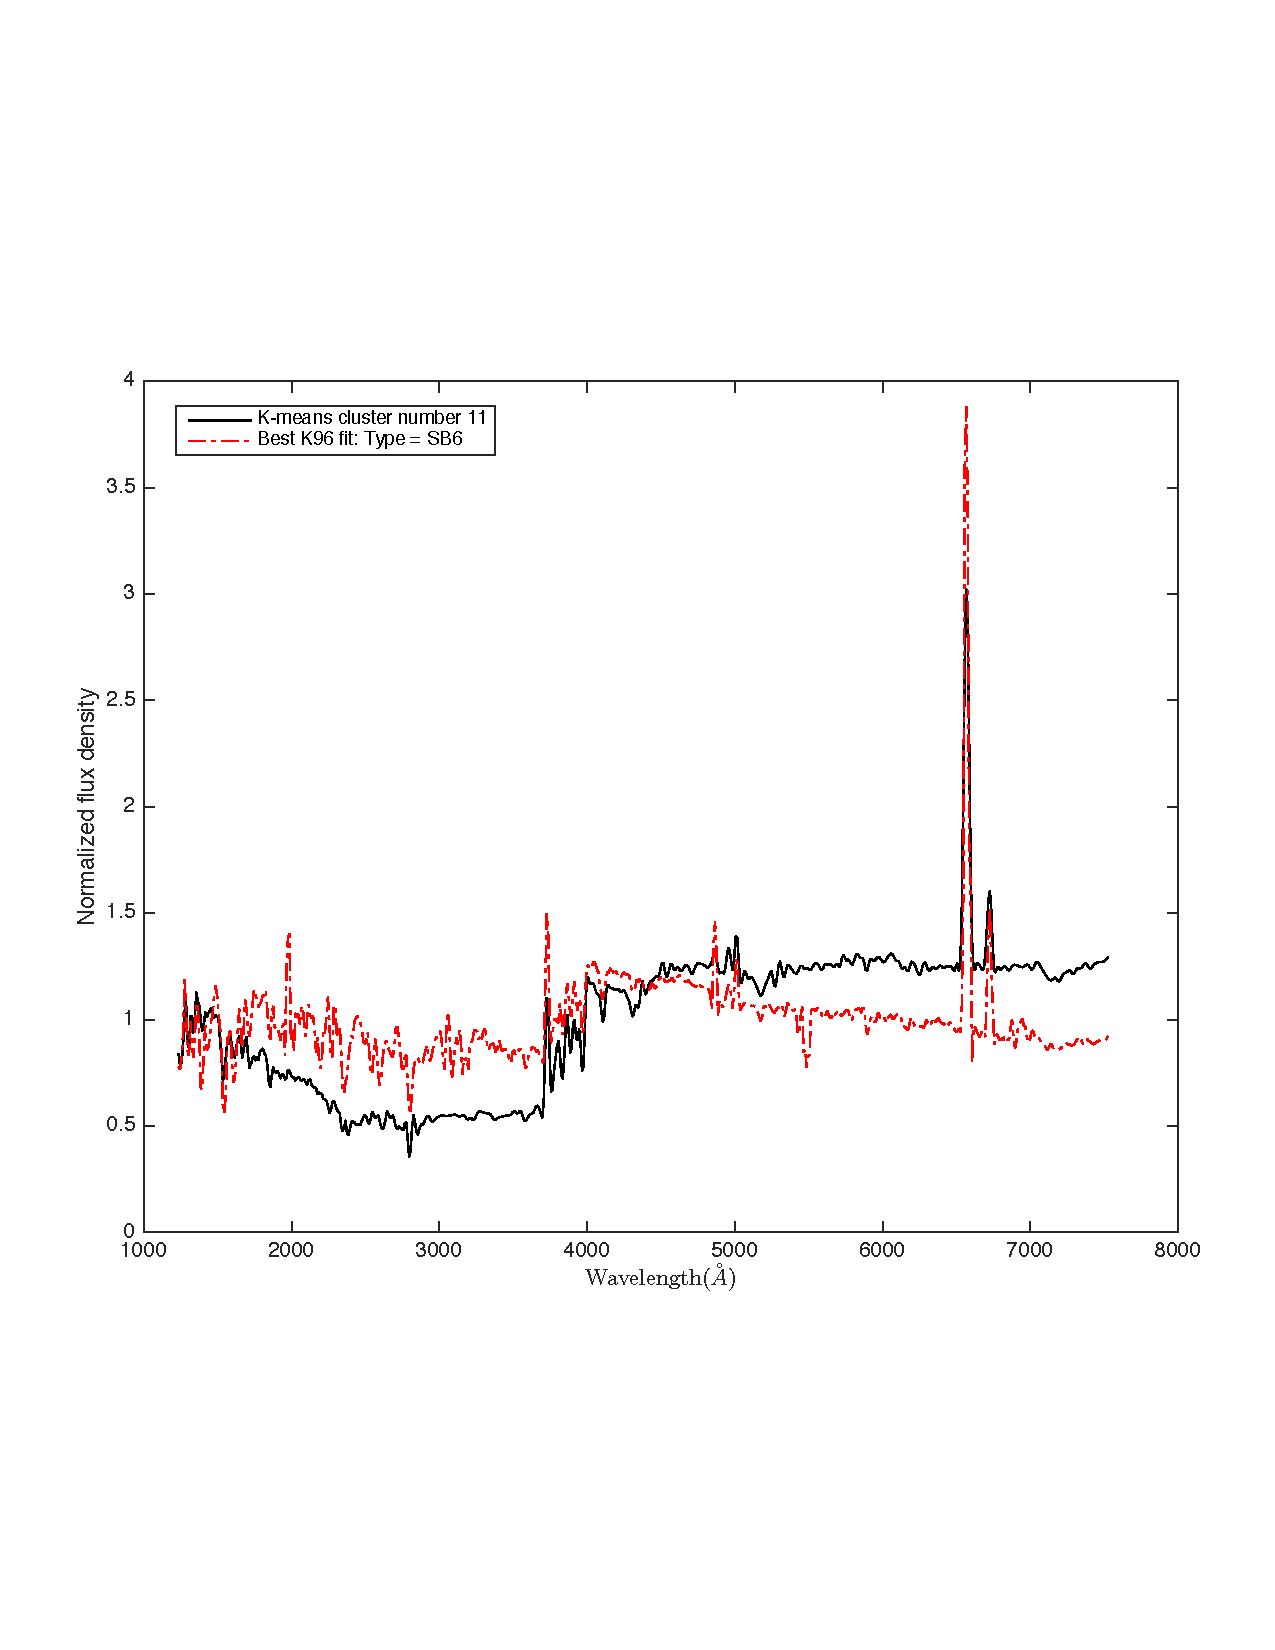
\includegraphics[width=.99\textwidth, height= 7.5cm]{k_means_images/max_cosine2.pdf}
                \end{subfigure}
                \hfill
                \begin{subfigure}[b]{0.49\textwidth}
                    \centering 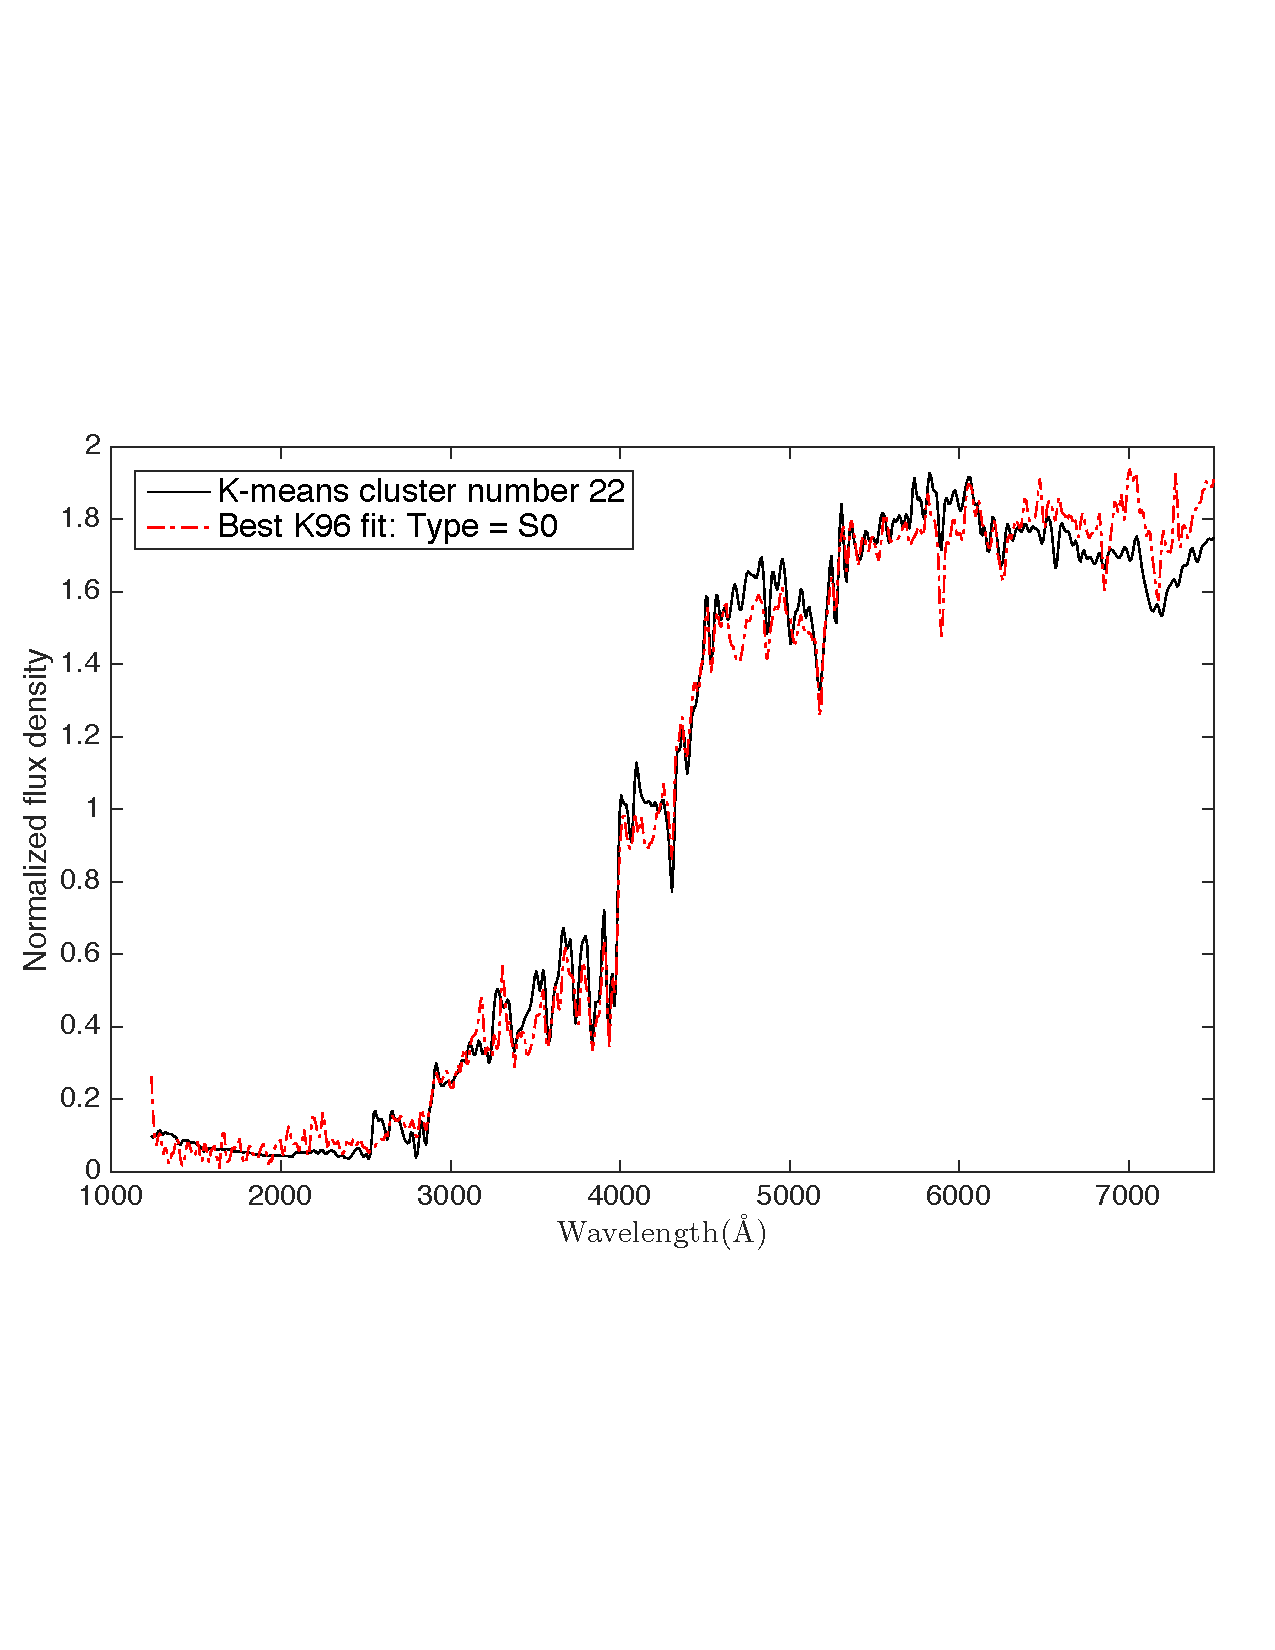
\includegraphics[width=.99\textwidth, height= 7.5cm]{k_means_images/min_cosine2.pdf}
                \end{subfigure}
                \caption{Left: the best match of \citetalias{Kinney96} templates for the median spectra of members in the cluster number 11. This fit has the maximum 1-$cos(\theta)$ among all 22 clusters. Right: the best fit of the \citetalias{Kinney96} templates to the median spectra in the  cluster number 17. This the best fitting result for 22 clusters.}
                 \label{fig: k_means_minmax}
\end{figure*}
For analyzing 142 sample galaxies from \citetalias{Hossein12}, we chose number of clusters for the K-means analysis to be 22.
The median spectra of the members of each cluster were fitted by a spectrum from the \citetalias{Kinney96} templates.
Although the K-means clustering method separated the spectra of 142 sample galaxies into 22 different groups, only 7 of template spectra matches the best with these 22 groups (some of the groups are classified as the same spectra type).
%As it is clear in Fig.~\ref{fig: k_means_minmax}, in some cases even the most similar template spectra is not a good fit to the median spectra of the clusters.
Fig.~\ref{fig: k_means_minmax}, shows the best and the worst fitting results among the 22 clusters. 
As we expected from the results of Section~\ref{sec: 1Dv} and \citetalias{Hossein12} paper, we cannot classify all the 142 sample galaxies with exactly 12 templates. 
Some of the classifications are almost perfect match, and there are group of galaxies that not exactly the same as any of the template spectra, but not completely different from them. 
The right plot in the Fig.~\ref{fig: k_means_minmax} is an example of group of galaxies that can not be consider as outlier (in the sense that they are not a completely different group of galaxies), but they cannot be matched exactly with any of the template spectra.

Being limited to the template is one of the disadvantages of the K-means algorithm over the SOM method. 
As mentioned in Sections~\ref{sec: 1Dv} and\ref{sec: 2D}, by performing SOM method on the template spectra, we create networks of neurons which each neurons either represents one of the spectrum from the template spectra or a spectrum that has (dis-)similarity with any of the template spectra. 
We can say that using SOM, we introduced a new template based on the \citetalias{Kinney96} template spectra, and classified the 142 sample galaxies based on this new template.

We classified 5 out of 22 clusters, 42 galaxies in total, from the K-means clustering as Sa type galaxies and 7 clusters, 28 galaxies in total, as SB1 type galaxies.
Using SOM method (see Fig.~\ref{fig: 1by22V}, only 19 galaxies were classified as Sa and 19 galaxies were classified as SB1. 
Fig.~\ref{fig: som_k_means_comp} shows the comparison between the median of the spectra classified by SOM and by K-means clustering. 
The medians of both spectra from both methods are tracing each other undoubtedly.
However, the normalized flux in each case is slightly different. 
For SB1 galaxies, flux at the low wavelength regime is lower for the K-means clusters than the SOM ones, and in the longer wavelengths the flux is higher.
These differences is reversed for Sa galaxies.

Using K-means clustering, no cluster were classified as Sb or SB2, which have very similar spectra to Sa and SB1, respectively.
On the other hand, 14 galaxies were recognized to have similar spectra to SB2, and 33 galaxies were recognized to have a spectra similar to Sa or Sb, using SOM method.
The differences in the classification and ignoring the templates with similar spectra might come from the error in K-means clustering or error in fitting problem.
In either case we can conclude that SOM method classifies galaxies considering more details than K-means clustering method. 




\begin{figure*}
                \begin{subfigure}[b]{0.49\textwidth}
                    \centering
                  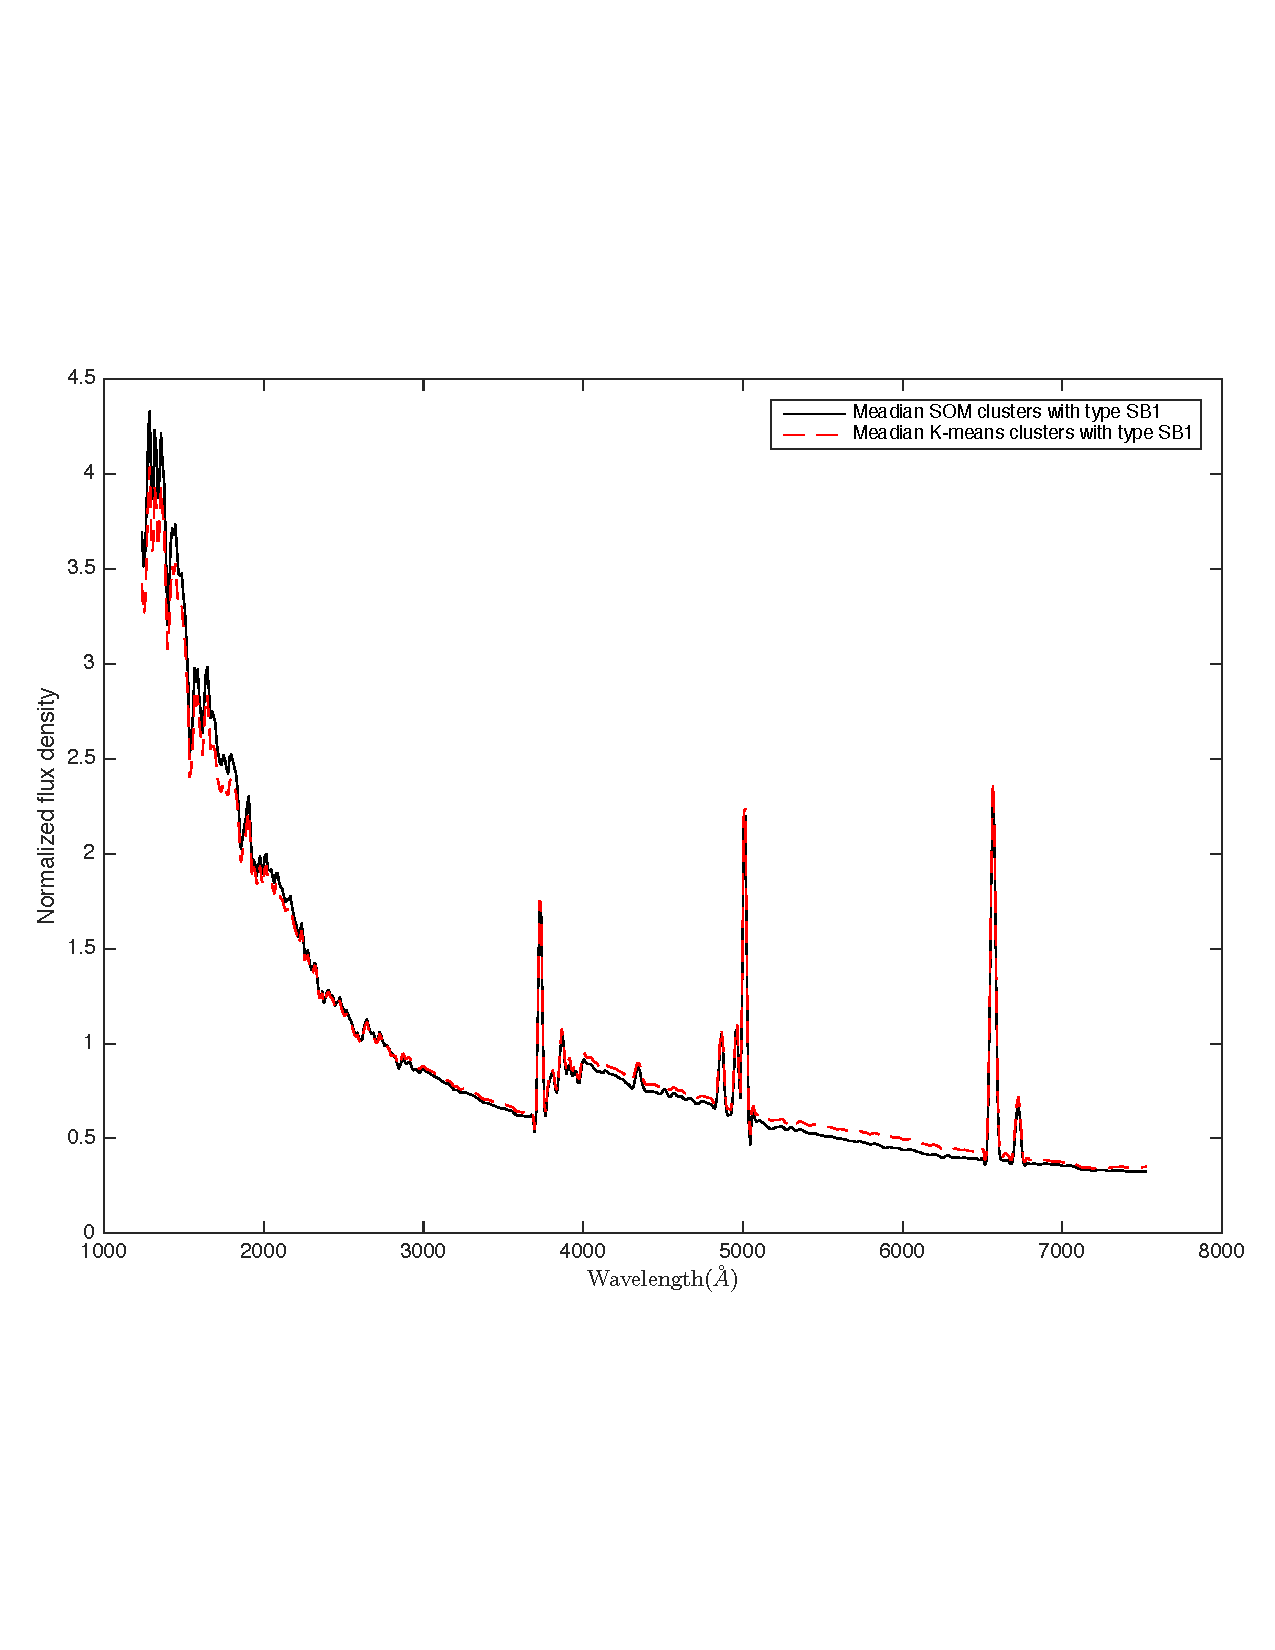
\includegraphics[width=0.99\textwidth, height= 7.5cm]{k_means_images/SB1_comp.pdf}
                \end{subfigure}
                \hfill
                \begin{subfigure}[b]{0.49\textwidth}
                    \centering 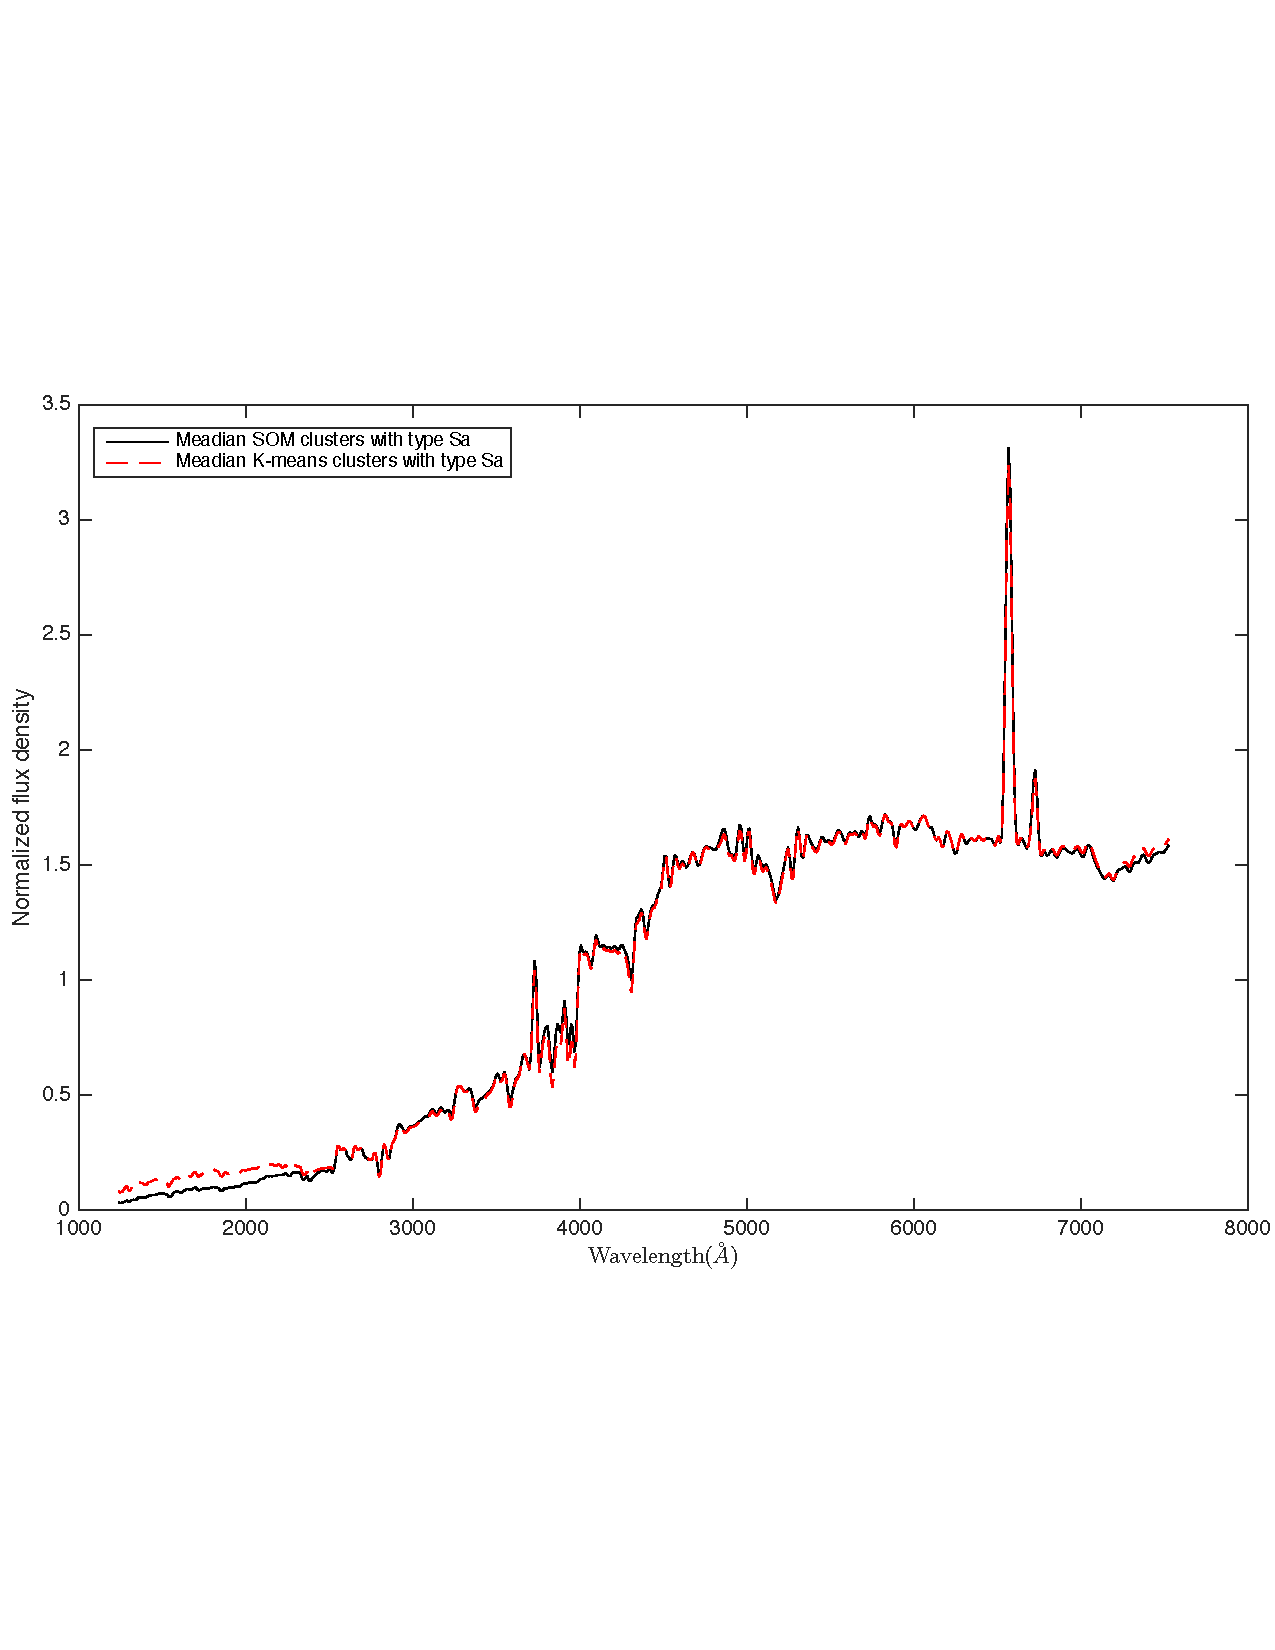
\includegraphics[width=\textwidth, height= 7.5cm]{k_means_images/Sa_comp.pdf}
                \end{subfigure}
                \caption{Comparing median of classified clusters from the K-means (dashed red lines) and SOM (solid black lines) methods. Left: the clusters in both method that is classified as SB1. Right: he clusters in both method that is classified as Sa.}
                 \label{fig: som_k_means_comp}
\end{figure*}

